% Options for packages loaded elsewhere
\PassOptionsToPackage{unicode}{hyperref}
\PassOptionsToPackage{hyphens}{url}
\PassOptionsToPackage{dvipsnames,svgnames,x11names}{xcolor}
%
\documentclass[
]{interact}

\usepackage{amsmath,amssymb}
\usepackage{iftex}
\ifPDFTeX
  \usepackage[T1]{fontenc}
  \usepackage[utf8]{inputenc}
  \usepackage{textcomp} % provide euro and other symbols
\else % if luatex or xetex
  \usepackage{unicode-math}
  \defaultfontfeatures{Scale=MatchLowercase}
  \defaultfontfeatures[\rmfamily]{Ligatures=TeX,Scale=1}
\fi
\usepackage{lmodern}
\ifPDFTeX\else  
    % xetex/luatex font selection
\fi
% Use upquote if available, for straight quotes in verbatim environments
\IfFileExists{upquote.sty}{\usepackage{upquote}}{}
\IfFileExists{microtype.sty}{% use microtype if available
  \usepackage[]{microtype}
  \UseMicrotypeSet[protrusion]{basicmath} % disable protrusion for tt fonts
}{}
\makeatletter
\@ifundefined{KOMAClassName}{% if non-KOMA class
  \IfFileExists{parskip.sty}{%
    \usepackage{parskip}
  }{% else
    \setlength{\parindent}{0pt}
    \setlength{\parskip}{6pt plus 2pt minus 1pt}}
}{% if KOMA class
  \KOMAoptions{parskip=half}}
\makeatother
\usepackage{xcolor}
\setlength{\emergencystretch}{3em} % prevent overfull lines
\setcounter{secnumdepth}{5}
% Make \paragraph and \subparagraph free-standing
\makeatletter
\ifx\paragraph\undefined\else
  \let\oldparagraph\paragraph
  \renewcommand{\paragraph}{
    \@ifstar
      \xxxParagraphStar
      \xxxParagraphNoStar
  }
  \newcommand{\xxxParagraphStar}[1]{\oldparagraph*{#1}\mbox{}}
  \newcommand{\xxxParagraphNoStar}[1]{\oldparagraph{#1}\mbox{}}
\fi
\ifx\subparagraph\undefined\else
  \let\oldsubparagraph\subparagraph
  \renewcommand{\subparagraph}{
    \@ifstar
      \xxxSubParagraphStar
      \xxxSubParagraphNoStar
  }
  \newcommand{\xxxSubParagraphStar}[1]{\oldsubparagraph*{#1}\mbox{}}
  \newcommand{\xxxSubParagraphNoStar}[1]{\oldsubparagraph{#1}\mbox{}}
\fi
\makeatother


\providecommand{\tightlist}{%
  \setlength{\itemsep}{0pt}\setlength{\parskip}{0pt}}\usepackage{longtable,booktabs,array}
\usepackage{calc} % for calculating minipage widths
% Correct order of tables after \paragraph or \subparagraph
\usepackage{etoolbox}
\makeatletter
\patchcmd\longtable{\par}{\if@noskipsec\mbox{}\fi\par}{}{}
\makeatother
% Allow footnotes in longtable head/foot
\IfFileExists{footnotehyper.sty}{\usepackage{footnotehyper}}{\usepackage{footnote}}
\makesavenoteenv{longtable}
\usepackage{graphicx}
\makeatletter
\newsavebox\pandoc@box
\newcommand*\pandocbounded[1]{% scales image to fit in text height/width
  \sbox\pandoc@box{#1}%
  \Gscale@div\@tempa{\textheight}{\dimexpr\ht\pandoc@box+\dp\pandoc@box\relax}%
  \Gscale@div\@tempb{\linewidth}{\wd\pandoc@box}%
  \ifdim\@tempb\p@<\@tempa\p@\let\@tempa\@tempb\fi% select the smaller of both
  \ifdim\@tempa\p@<\p@\scalebox{\@tempa}{\usebox\pandoc@box}%
  \else\usebox{\pandoc@box}%
  \fi%
}
% Set default figure placement to htbp
\def\fps@figure{htbp}
\makeatother
% definitions for citeproc citations
\NewDocumentCommand\citeproctext{}{}
\NewDocumentCommand\citeproc{mm}{%
  \begingroup\def\citeproctext{#2}\cite{#1}\endgroup}
\makeatletter
 % allow citations to break across lines
 \let\@cite@ofmt\@firstofone
 % avoid brackets around text for \cite:
 \def\@biblabel#1{}
 \def\@cite#1#2{{#1\if@tempswa , #2\fi}}
\makeatother
\newlength{\cslhangindent}
\setlength{\cslhangindent}{1.5em}
\newlength{\csllabelwidth}
\setlength{\csllabelwidth}{3em}
\newenvironment{CSLReferences}[2] % #1 hanging-indent, #2 entry-spacing
 {\begin{list}{}{%
  \setlength{\itemindent}{0pt}
  \setlength{\leftmargin}{0pt}
  \setlength{\parsep}{0pt}
  % turn on hanging indent if param 1 is 1
  \ifodd #1
   \setlength{\leftmargin}{\cslhangindent}
   \setlength{\itemindent}{-1\cslhangindent}
  \fi
  % set entry spacing
  \setlength{\itemsep}{#2\baselineskip}}}
 {\end{list}}
\usepackage{calc}
\newcommand{\CSLBlock}[1]{\hfill\break\parbox[t]{\linewidth}{\strut\ignorespaces#1\strut}}
\newcommand{\CSLLeftMargin}[1]{\parbox[t]{\csllabelwidth}{\strut#1\strut}}
\newcommand{\CSLRightInline}[1]{\parbox[t]{\linewidth - \csllabelwidth}{\strut#1\strut}}
\newcommand{\CSLIndent}[1]{\hspace{\cslhangindent}#1}

\usepackage{booktabs}
\usepackage{caption}
\usepackage{longtable}
\usepackage{colortbl}
\usepackage{array}
\usepackage{anyfontsize}
\usepackage{multirow}
\usepackage{orcidlink}
\makeatletter
\@ifpackageloaded{tcolorbox}{}{\usepackage[skins,breakable]{tcolorbox}}
\@ifpackageloaded{fontawesome5}{}{\usepackage{fontawesome5}}
\definecolor{quarto-callout-color}{HTML}{909090}
\definecolor{quarto-callout-note-color}{HTML}{0758E5}
\definecolor{quarto-callout-important-color}{HTML}{CC1914}
\definecolor{quarto-callout-warning-color}{HTML}{EB9113}
\definecolor{quarto-callout-tip-color}{HTML}{00A047}
\definecolor{quarto-callout-caution-color}{HTML}{FC5300}
\definecolor{quarto-callout-color-frame}{HTML}{acacac}
\definecolor{quarto-callout-note-color-frame}{HTML}{4582ec}
\definecolor{quarto-callout-important-color-frame}{HTML}{d9534f}
\definecolor{quarto-callout-warning-color-frame}{HTML}{f0ad4e}
\definecolor{quarto-callout-tip-color-frame}{HTML}{02b875}
\definecolor{quarto-callout-caution-color-frame}{HTML}{fd7e14}
\makeatother
\makeatletter
\@ifpackageloaded{caption}{}{\usepackage{caption}}
\AtBeginDocument{%
\ifdefined\contentsname
  \renewcommand*\contentsname{Table of contents}
\else
  \newcommand\contentsname{Table of contents}
\fi
\ifdefined\listfigurename
  \renewcommand*\listfigurename{List of Figures}
\else
  \newcommand\listfigurename{List of Figures}
\fi
\ifdefined\listtablename
  \renewcommand*\listtablename{List of Tables}
\else
  \newcommand\listtablename{List of Tables}
\fi
\ifdefined\figurename
  \renewcommand*\figurename{Figure}
\else
  \newcommand\figurename{Figure}
\fi
\ifdefined\tablename
  \renewcommand*\tablename{Table}
\else
  \newcommand\tablename{Table}
\fi
}
\@ifpackageloaded{float}{}{\usepackage{float}}
\floatstyle{ruled}
\@ifundefined{c@chapter}{\newfloat{codelisting}{h}{lop}}{\newfloat{codelisting}{h}{lop}[chapter]}
\floatname{codelisting}{Listing}
\newcommand*\listoflistings{\listof{codelisting}{List of Listings}}
\makeatother
\makeatletter
\makeatother
\makeatletter
\@ifpackageloaded{caption}{}{\usepackage{caption}}
\@ifpackageloaded{subcaption}{}{\usepackage{subcaption}}
\makeatother

\usepackage{bookmark}

\IfFileExists{xurl.sty}{\usepackage{xurl}}{} % add URL line breaks if available
\urlstyle{same} % disable monospaced font for URLs
\hypersetup{
  pdftitle={Muslim Diversity Study: Quantitative protocol and practical insights on engaging New Zealand's Muslim communities},
  pdfauthor={M. Usman Afzali; Jamila S. Badis; Parus Khoso; Gul e Aqsa; Mazharuddin Syed Ahmed; Aamina Ali; Afrah Ali; Zarqa Shaheen Ali; Ayca Arkilic; Tuba Azeem; Hala Burhoum; Zahra Emamzadeh; Zahra Haidary; Nasratullah Hamid; Iman Husain; Fatima A. Junaid; Mashal Khan; Adepate Mustapha-Koiki; Hussain Raissi; Farah Shawkat; Rizwan Sulehry; Mai Tamimi; Sandila Tanveer; Somia Tasneem; Kumar Yogeeswaran; Chris G. Sibley; Joseph A. Bulbulia; Aarif A. Rasheed},
  pdfkeywords={Muslims, diversity, New Zealand Attitudes and Values
Study, Muslim Diversity Study, New Zealand},
  colorlinks=true,
  linkcolor={blue},
  filecolor={Maroon},
  citecolor={Blue},
  urlcolor={Blue},
  pdfcreator={LaTeX via pandoc}}


\title{Muslim Diversity Study: Quantitative protocol and practical
insights on engaging New Zealand's Muslim communities}
\author{M. Usman
Afzali$\textsuperscript{1,2}$~\orcidlink{0000-0001-5119-9388}, Jamila S.
Badis$\textsuperscript{2}$~\orcidlink{0009-0005-2866-5033}, Parus
Khoso$\textsuperscript{3}$~\orcidlink{0000-0001-6384-038X}, Gul e
Aqsa$\textsuperscript{4}$~\orcidlink{0009-0003-0928-8039}, Mazharuddin
Syed Ahmed$\textsuperscript{5}$~\orcidlink{0009-0006-9799-4049}, Aamina
Ali$\textsuperscript{6}$~\orcidlink{0009-0000-8153-8432}, Afrah
Ali$\textsuperscript{7}$~\orcidlink{0009-0004-5856-4025}, Zarqa Shaheen
Ali$\textsuperscript{8}$~\orcidlink{0000-0002-7145-5788}, Ayca
Arkilic$\textsuperscript{9}$~\orcidlink{0000-0002-1775-3311}, Tuba
Azeem$\textsuperscript{10}$~\orcidlink{0000-0002-0611-8726}, Hala
Burhoum$\textsuperscript{2}$~\orcidlink{0009-0004-3867-2029}, Zahra
Emamzadeh$\textsuperscript{11}$~\orcidlink{0009-0007-3065-2199}, Zahra
Haidary$\textsuperscript{2}$~\orcidlink{0009-0000-5259-622X}, Nasratullah
Hamid$\textsuperscript{12}$~\orcidlink{0009-0002-0120-7428}, Iman
Husain$\textsuperscript{2}$~\orcidlink{0000-0003-4032-4387}, Fatima A.
Junaid$\textsuperscript{13}$~\orcidlink{0000-0002-6656-8120}, Mashal
Khan$\textsuperscript{2}$~\orcidlink{0009-0004-5903-3306}, Adepate
Mustapha-Koiki$\textsuperscript{14}$~\orcidlink{0000-0003-4731-1781}, Hussain
Raissi$\textsuperscript{15}$~\orcidlink{0009-0000-7985-1622}, Farah
Shawkat$\textsuperscript{1}$~\orcidlink{0009-0006-0319-9117}, Rizwan
Sulehry$\textsuperscript{16}$~\orcidlink{0000-0002-1209-0635}, Mai
Tamimi$\textsuperscript{7}$~\orcidlink{0009-0001-7894-7259}, Sandila
Tanveer$\textsuperscript{12}$~\orcidlink{0000-0002-0648-5382}, Somia
Tasneem$\textsuperscript{17}$~\orcidlink{0000-0001-5471-6934}, Kumar
Yogeeswaran$\textsuperscript{2}$~\orcidlink{0000-0002-1978-5077}, Chris
G. Sibley$\textsuperscript{18}$~\orcidlink{0000-0002-4064-8800}, Joseph
A.
Bulbulia$\textsuperscript{19,20}$~\orcidlink{0000-0002-5861-2056}, Aarif
A. Rasheed$\textsuperscript{21}$~\orcidlink{0009-0004-7513-430X}}

\thanks{CONTACT: M. Usman
Afzali. Email: \href{mailto:usman.afzali@otago.ac.nz}{\nolinkurl{usman.afzali@otago.ac.nz}}. }
\begin{document}
\captionsetup{labelsep=space}
\maketitle
\textsuperscript{1} Religion Programme, University of
Otago,  \\ \textsuperscript{2} School of Psychology, Speech and
Hearing, University of Canterbury,  \\ \textsuperscript{3} College of
Education, University of Canterbury,  \\ \textsuperscript{4} School of
Health Sciences, University of
Canterbury,  \\ \textsuperscript{5} Engineering and Architectural
Studies, Ara Institute of
Canterbury,  \\ \textsuperscript{6}  PsychologyNZ,  \\ \textsuperscript{7}  Independent
Researcher,  \\ \textsuperscript{8} ICL Business School, New Zealand
Skills and Education College,  \\ \textsuperscript{9} School of History,
Philosophy, Political Science and International Relations, Victoria
University of Wellington,  \\ \textsuperscript{10} Faculty of
Law, Victoria University of Wellington,  \\ \textsuperscript{11} School
of Language, Social \& Political Sciences, University of
Canterbury,  \\ \textsuperscript{12} Department of Psychological
Medicine, University of Otago
Christchurch,  \\ \textsuperscript{13} School of Management, Massey
University,  \\ \textsuperscript{14} Department of Politics and
International Relations, University of
Auckland,  \\ \textsuperscript{15} The National Centre for Peace and
Conflict Studies, University of Otago,  \\ \textsuperscript{16} School
of Management, Victoria University of
Wellington,  \\ \textsuperscript{17} Department of History, Government
College University, Faisalabad,
Pakistan,  \\ \textsuperscript{18} School of Psychology, University of
Auckland,  \\ \textsuperscript{19} School of Psychology, Victoria
University of Wellington,  \\ \textsuperscript{20} Department of
Linguistic and Cultural Evolution, Max Planck Institute for Evolutionary
Anthropology,  \\ \textsuperscript{21}  Just Community,  
\begin{abstract}
The New Zealand Attitudes and Values Study (NZAVS) is a national
longitudinal study aiming to understand social values and attitudes in
New Zealanders by tracking responses in the same people over time.
Previously, the NZAVS has been undersampling Muslims by ten times lower
than those of other religious groups. The Muslim Diversity Study
recruits a proportionately representative cohort of Muslims to involve
them in longitudinal scientific research within NZAVS. With this, we
hope that the stories of Muslim adversity and resilience will be more
accurately recorded and understood. Such inclusion enriches the
scientific study of human flourishing, addresses the curiosity of the
Muslim community in understanding its diversity, and contributes
practical insights that can lead to the betterment of this marginalised
community. We describe the motivations for the study, explain how the
study was developed in consultation with the community, outline our
methods, and offer practical guidelines for data collection from a
culturally diverse community. In the first instance, this article offers
a record of our research with Muslims in New Zealand. We hope this will
prove useful to investigators seeking to understanding human flourishing
in other settings through the national-scale longitudinal study of
culturally diverse, marginalised religious communities.
\end{abstract}
\begin{keywords}
\def\sep{;\ }
Muslims\sep diversity\sep New Zealand Attitudes and Values
Study\sep Muslim Diversity Study\sep 
New Zealand
\end{keywords}


\section{Introduction}\label{sec-intro}

Officially known as \emph{A national longitudinal study of Muslim
diversity and flourishing}, the Muslim Diversity Study (MDS) embraces a
community-oriented approach by collaborating with the Muslim community
in order to make decisions about the execution of data collection and
for identifying key questions of interest for the community at large. It
is important that such processes and decisions are recorded in the form
of an article so that our findings and recommendations are shared with
the broader public and future researchers in New Zealand and across the
globe.

MDS started in 2023 as part of the New Zealand Attitudes and Values
Study (NZAVS). The NZAVS is a planned 20-year-long longitudinal national
probability annual panel study of social attitudes, personality,
ideology and health outcomes that began in 2009 and is currently in its
16th year. It has so far collected data from more than 70,000 New
Zealand residents using the electoral roll (Sibley 2024). The NZAVS has
been instrumental in exploring key issues related to minorities,
including but not limited to discrimination, intergroup relations,
identity, distress, security, and the dynamics and mechanisms behind
them.

The NZAVS has been uniquely positioned due to its prestigious reputation
(over 300 peer-reviewed publications), longitudinal panel design, large
sample size, and a large multi-disciplinary research team (Sibley 2024).
More importantly, NZAVS has a nationally representative sample with data
from different identity and religious groups (Sibley 2024), thereby
allowing researchers to compare data from different identity groups.
However, the NZAVS has been undersampling Muslims by ten times lower
than those of other religious groups (Sibley 2024), which did not allow
us to make meaningful inferences regarding Muslim lives and issues in
comparison with other religious groups. Hence, the goal of MDS is to
achieve as many as 650 Muslim respondents (i.e., \textasciitilde{} 1\%
of the total nation's Muslim community).

This article has three major parts. After providing the broader context
of Muslims and MDS, we firstly discuss the process of co-designing and
adjustments to the NZAVS design. Secondly, we present the final design
and implemented protocol. Thirdly, we share the summary of advice and
lessons learned in the process.

\section{Muslims in New Zealand}\label{muslims-in-new-zealand}

The Muslim community has been expanding in New Zealand. Based on the
2018 census, New Zealand had more than 60,000 Muslims which has grown to
over 75,000 according to the 2023 Census ({``Stats NZ''} 2024). Studies
also show that the number of converts to Islam has recently increased
(Arkilic 2020). The Muslim community is uniquely positioned in New
Zealand: a growing religious minority and a historically stigmatised
group that was the direct target of the 15 March 2019 terrorist attack
({``Royal {C}ommission of {I}nquiry into the Terrorist Attack on
{C}hristchurch {M}asjidain on 15 {M}arch 2019''} 2020; Sibley et al.
2020).

The devastating far-right extremist attack on two mosques took place in
Christchurch, killing 51 Muslims and injuring 40 ({``Royal {C}ommission
of {I}nquiry into the Terrorist Attack on {C}hristchurch {M}asjidain on
15 {M}arch 2019''} 2020). Although this attack was widely condemned
({``World Leaders Condemn New Zealand Mosque Attacks''} 2019) and was
unprecedented in New Zealand ({``Jacinda {A}rdern on the {C}hristchurch
Shooting: {`}One of {N}ew {Z}ealand's Darkest Days'''} 2019), it was not
as surprising to the Muslim community (A. Rahman 2019). Leading up to
the attacks, many Muslims had regularly experienced Islamophobia and
prejudice (Sibley et al. 2020; Shaver et al. 2017, 2016).

Even as Islamophobia has reportedly increased overseas following these
attacks ({``Islamophobia After {C}hristchurch Terror Attacks Quadrupled
- {A}ustralian Report''} 2022), the evidence in New Zealand seems to be
mixed. While news articles have reported increased hate (Frykberg 2023),
the NZAVS findings were indicative of improved attitudes towards Muslims
(Shanaah et al. 2021; Bulbulia et al. 2023) following the attacks.
Addressing this discrepancy is beyond the scope of the current article;
however, it is worth noting that most of our research in this area,
primarily through the NZAVS lens, has so far shed light on such
attitudes from a non-Muslim perspective. In other words, we have mostly
reported on how Muslims are perceived by non-Muslim members of New
Zealand society, rather than how Muslims perceive themselves. Although
NZAVS studies of anti-Muslim prejudice are scientifically important,
systematic insights into how Muslims are diversely responding to
prejudice, and where Muslims are diversely found resilience remain
unclear.

Muslims have generally faced prejudicial attitudes in New Zealand
(Yogeeswaran et al. 2019; Sibley et al. 2020; Greaves et al. 2020).
Until the Christchurch terror attack, news stories on Islam and Muslims
in New Zealand media were mostly an extension of `the negative othering
rhetoric', and the national media tended to link Muslim converts to
jihadis (Drury 2016). Unsurprisingly, such rhetoric has been found to
foster anti-Muslim prejudice (Shaver et al. 2017).

In the aftermath of Christchurch shootings, the New Zealand government
introduced unprecedented counter-terrorism measures such as the
prohibition of the sale of all military-style semi-automatic and assault
rifles and creating the Royal Commission of Inquiry into these attacks
({``Royal {C}ommission of {I}nquiry into the Terrorist Attack on
{C}hristchurch {M}asjidain on 15 {M}arch 2019''} 2020). The Royal
Commission of Inquiry presented an 800-page report emphasising New
Zealand's inclusive and welcoming identity, among other measures
(Arkilic 2021). In addition, the New Zealand press embraced a more
inclusive and positive narrative with respect to Islam and Muslims (K.
A. Rahman 2020; Kabir 2024).

In summary, although there have been sporadic reports of increased hate
crimes after the attacks (Wilson and Shastri 2020), the average
sentiments towards Muslims have improved in New Zealand. The NZAVS, in a
series of articles, reported this positive shift in these attitudes
toward Muslims post Christchurch attacks (Shanaah et al. 2021; Bulbulia
et al. 2023), and the psychological response of New Zealand public to
the shootings (Byrne et al. 2022).

The Christchurch shootings prompted many New Zealand research groups and
institutions to further study about Muslims and with Muslims, who so far
had been a culturally-distinct, under-researched, minority group. These
studies included trauma-focused response (Sulaiman-Hill et al. 2021;
Sulaiman-Hill, Porter, et al. 2024), inclusion, Islamophobia and
wellbeing (Junaid, Cassim, and Khan-Janif 2024), perceived
discrimination among Muslim immigrant youth (Raissi 2024), the political
implications of government decisions (Arkilic 2021) among others. Given
that the NZAVS had explored perceptions of Muslims and the mechanisms of
attitudinal changes towards Muslims following 15 March 2019 attacks
(Sibley et al. 2020; Shaver et al. 2017; Bulbulia et al. 2023; Hawi et
al. 2019), it was a timely necessity that we expanded our reach to focus
on the experiences of this same group.

In addition, much of the NZAVS work to date with the Muslim community
had focused on conveying information about how Muslims are perceived by
the non-Muslim members of New Zealand society. After receiving strong
positive suggestions from the Muslim community to scientifically explore
diversity, discrimination, self-perception, resilience, meaning-making
and flourishing, the MDS was conceptualised in 2022 to address this
scholarly and community knowledge gap. Therefore, MDS is effectively a
booster to NZAVS, and uses the NZAVS questionnaires to collect data from
the members of Muslim community in New Zealand.

Media reports pointed out incredible resilience and flourishing of
victims as well as the wider Muslim community post Christchurch
shootings (Oliver 2024; Greenfield 2019). Limited research on specific
cohorts of Muslims indicated the same (Sulaiman-Hill, Schluter, et al.
2024; Nasier 2023). Research on human flourishing has consistently shown
that religiosity and religious service attendance might be associated
with various aspects of human flourishing (VanderWeele 2017a, 2017b).
New Zealand Muslims' overall under-representation in research and
resilience in the face of prejudice and terror produced a critical
research gap in the relationship of Muslim religiosity and flourishing
that warranted further empirical investigation. By addressing this line
of inquiry with MDS, we contribute to the science of human flourishing
in general.

\section{MDS research aims}\label{mds-research-aims}

MDS aims to investigate the role of religious community engagement in
buffering Muslims against anti-Muslim prejudice, to examine the
employment and health challenges faced by Muslims relative to other
religious groups, and to explore the similarities in subjective
wellbeing and psychological distress across religious affiliations,
emphasising the protective effects of community support and religious
community-making. In addition, we aim to explore the diversity of
Muslims in New Zealand, assess Muslims' perceived discrimination in
comparison with other religious groups, unearth predictors of their
flourishing and meaning-making, and measure the effect of
service-attendance and religious-identification on these constructs.
This comprehensive approach enables the examination of both direct
relationships and complex mediating pathways between religious community
engagement, experienced prejudice, employment and health outcomes, and
psychological wellbeing. Through this multifaceted investigation, the
study seeks to contribute to our understanding of the Muslim experience
in New Zealand and the role of religious community support in promoting
positive outcomes across various life domains.

\section{Part 1: Co-designing}\label{part-1-co-designing}

\subsection{Community consultation}\label{community-consultation}

Prior to applying for the research grant, we deemed it necessary to
consult with the Muslim community to gauge interest in the project, and
the feasibility of the project for the community. More importantly,
inferring from the culturally-focused research groups, it was important
to co-design the project with Muslims by consulting with the academics
and leaders of the Muslim community. Therefore, the principal
investigator (MUA) started engaging with the Muslim community in
February 2022 --- one year before the start of the project --- to
co-design the project.

This consultation continued until November 2022, where MUA reached out
to 29 Muslims in six cities, Auckland, Hamilton, Palmerston North,
Wellington, Christchurch, and Dunedin, from various age groups, genders,
and cultural backgrounds. Twenty of these conversations took place with
community leaders, religious scholars, academics, and cultural leaders,
while 9 conversations took place with individual activists. The
conversations were focused around four objectives: 1) To assess the
feasibility of the project for Muslims, 2) To assess the interest of
Muslims in the project, 3) To get feedback on the survey items, design,
and working with the community, and 4) To inquire if translation of the
questionnaire may be needed. The consultation revealed unanimous
agreement among respondents regarding the study's feasibility and
timeliness for the Muslim community, with expectations of strong
interest in participation. The respondents indicated that the highest
engagement would likely come from youth groups, subsequent-generation
migrants, those with formal education, and female participants.
Furthermore, the respondents not only endorsed the significance of the
study and its planned measures but also pledged their comprehensive
support for the initiative.

A few challenges were also identified with regards to the execution of
the study: 1) The participation from Christchurch might not be up to the
anticipated levels as after the Christchurch shooting, people were
frequently surveyed and not provided with the findings, which might have
affected their interest to participate in the study. 2) It might not be
easy for all prospective participants to understand the questionnaires
due to the community's unfamiliarity with research and limitations with
fluency in English. 3) The participation from the elderly community (due
to unfamiliarity with research) and Muslim converts (due to distrust of
the institutions) might also be low. 4) Community members might be
suspicious and consider the study to have ulterior or personal motives.
Similar challenges have been identified by other researchers who have
worked with the Muslim community in New Zealand (Sulaiman-Hill, Porter,
et al. 2024).

The following recommendations on mitigating these challenges were
received upon completing the consultation: 1) To encourage more
participation from the Muslim community, findings should be shared with
the wider community in future owing to the diversity it will present. To
be able to share the research findings with the community smoothly and
keep them up-to-date, it was recommended to have a dedicated website for
the study. Therefore, instead of calling it a booster to NZAVS, the
project was named Muslim Diversity Study, and a website of the same name
was created. 2) Although many said that the questionnaire needs to be
translated into seven ethnic languages in connection to reducing the
difficulty in reaching the diverse members of the community for the
study, they also indicated that a majority of the potential participants
could comprehend the English version easily. 3) It was proposed that we
should reach out to the community via trusted community leaders/members,
ethnic and religious organisations, and mosques, and that for youth
engagement, we should go via youth organisations such as Muslim Student
Associations (MSAs) at universities. A family-focused strategy was
advised to be beneficial as starting with the men was implied to be more
effective. 4) To assuage the possible distrust around the motives of the
study, the participants must be clearly informed about the study's
rationale and its benefits to the community, reiterating that it will
increase Muslims' visibility and raise their voice in research. The
long-term value of the study for the community as a whole as well as
their children should also be emphasised.

This process led to the development of comprehensive guidelines that
address feasibility, advice on engagement with the community, the
possible challenges, and avenues to enhance participation. The 29
participants of this pilot consultation form the Advisory Group of MDS
and are being regularly consulted.

\subsection{Translation}\label{translation}

Our consultation with the community revealed that the need for
translation of the questionnaire may be limited to a small subset of New
Zealand Muslims, as the majority are expected to be proficient in
English. This finding aligns with the research conducted by the March 15
Project team (Sulaiman-Hill et al. 2021), which found that 71\% of
participants preferred English for surveys and clinical interviews.

A critical component of the MDS is the comparison of Muslim scores on
the NZAVS with those of other religious groups. The introduction of a
translated questionnaire poses the risk of not capturing attitudes and
behaviours with the same accuracy as the English version. Consequently,
any observed differences in scores between Muslims and other groups
could be attributed to translation bias rather than genuine differences
in religious affiliations.

This concern was presented to the Advisory Group, which recommended
against translating the questionnaire. Instead, it was advised to
provide the English version to all potential Muslim participants. This
approach offers a methodological safeguard, ensuring that the conceptual
meanings are preserved and not distorted by translation. By maintaining
the integrity of the questionnaire, we can be more confident in the
validity of the comparative analyses between religious groups.

\subsection{Item retention and religious Context
Considerations}\label{item-retention-and-religious-context-considerations}

The consultation process with the MDS Advisory Group identified six
items in the New NZAVS questionnaire that could potentially appear
irrelevant to Muslim participants, given the questionnaire's original
development within a predominantly Christian and secular context.
Despite these potential concerns, a substantial majority of the Advisory
Group (81\% average across all six items) recommended retaining these
items to enable meaningful cross-religious comparisons in the analysis.

To address potential participant concerns about item relevance, we
included in the survey instructions: ``As the survey is designed for the
general New Zealand population, there may be questions that do not
necessarily apply to you. Please feel free to skip any questions that
you do not wish to answer.'' This approach maintains methodological
consistency while acknowledging and accommodating the diverse religious
perspectives of participants.

\section{Part 2: Protocol}\label{part-2-protocol}

\subsection{Sample size estimation and
participants}\label{sample-size-estimation-and-participants}

The NZAVS sample of Muslim cohort was \emph{n} = 85 prior to MDS (Sibley
2024). To enhance the representation of Muslims in NZAVS, we initially
aimed to recruit an additional 1500 participants, more than doubling the
study's proportional sampling of the general population. We were able to
recruit \emph{n} = 582 new participants. This target corresponds to
about 1.3\% of New Zealand's Muslim population based on the 2018 Census
({``Stats NZ''} 2024). Notably, the 2023 Census that took place after
the start of MDS shows an increased number of Muslims in New Zealand
(75,138) ({``2023 {C}ensus {P}opulation, {D}welling, and {H}ousing
{H}ighlights''} 2024). Data collection was concentrated in six major
urban centers---Auckland, Christchurch, Hamilton, Wellington, Palmerston
North, and Dunedin---each with a Muslim population of at least 1,000
(see Table~\ref{tbl-muslim-population}). Participants were eligible if
they self-identify as Muslim, were 18 years or older, and currently
resided in New Zealand. There were no exclusion criteria. By conclusion
of Wave 15, the sample size of NZAVS is 32,857, with further details
available online (\url{https://osf.io/75snb/}). The total number of
Muslim participants in NZAVS Wave 15 is 667.

\begin{table}

\caption{\label{tbl-muslim-population}}

\centering{

\caption*{
{\large Muslim Population in 2022 by Selected Cities (From Stats NZ, 2024)}
} 
\fontsize{12.0pt}{14.4pt}\selectfont
\begin{tabular*}{\linewidth}{@{\extracolsep{\fill}}lrr}
\toprule
City & Population & Research Assistants \\ 
\midrule\addlinespace[2.5pt]
Auckland & 40,221 & 10 \\ 
Christchurch & 3,942 & 8 \\ 
Hamilton & 3,561 & 4 \\ 
Wellington & 3,294 & 5 \\ 
Palmerston North & 1,317 & 1 \\ 
Dunedin & 1,299 & 2 \\ 
\bottomrule
\end{tabular*}

}

\end{table}%

\subsection{Materials}\label{materials}

We are highlighting measures that are pertinent to the planned papers
aimed at communicating the findings emerging from MDS. The complete list
of NZAVS measures can be accessed online (\url{https://osf.io/75snb/}).

For Likert type scales, the minimum and maximum levels are noted along
with the description: for instance, 1 = Not Important, 7 = Very
Important would mean that a score ranges between 1 and 7, with 1 being
the minimum and 7 being the maximum score, whereas (R) indicates the
reverse-scored items. Notwithstanding, we might choose to explore
further measures which will then be elaborated on in the individual
articles.

\subsubsection{Service attendance and
religiosity}\label{service-attendance-and-religiosity}

\begin{enumerate}
\def\labelenumi{\arabic{enumi}.}
\tightlist
\item
  Do you identify with a religion and/or spiritual group? (Yes/No). If
  yes, what religion or spiritual group? (String entry).
\item
  How many times did you attend a church or place of worship in the last
  month? (String entry).
\item
  How many times did you pray in the last week? (String entry).
\item
  How many times did you read religious scripture in the last week?
  (String entry).
\item
  How important is your religion to how you see yourself? (1 = Not
  Important, 7 = Very Important).
\item
  I identify as a spiritual person. (1 = Strongly Disagree, 7 = Strongly
  Agree).
\item
  Do you believe in God? (Yes/No).
\item
  Do you believe in any form of spirit or life force? (Yes/No).
\end{enumerate}

\subsubsection{Prejudice}\label{prejudice}

\begin{enumerate}
\def\labelenumi{\arabic{enumi}.}
\tightlist
\item
  I feel that I am often discriminated against because of my
  religious/spiritual beliefs. (1 = Strongly Disagree, 7 = Strongly
  Agree).
\item
  People from my ethnic group are discriminated against in New Zealand.
  (1 = Strongly Disagree, 7 = Strongly Agree).
\item
  I feel that I am often discriminated against because of my age. (1 =
  Strongly Disagree, 7 = Strongly Agree).
\item
  I feel that I am often discriminated against because of my ethnicity.
  (1 = Very Inaccurate, 7 = Very Accurate).
\item
  I feel that I am often discriminated against because of my gender. (1
  = Very Inaccurate, 7 = Very Accurate).
\item
  Intergroup Warmth Ratings: Participants are asked to rate their
  feelings of warmth toward different groups using the ``Feeling
  Thermometer Scale'' for each group from least to most warmth on a
  7-point scale where 1 = Least Warm and 7 = Most Warm (see
  Figure~\ref{fig-warmth} for reference). Groups include NZ Europeans,
  Māori, Asians in general, Pacific Islanders, Elderly people, People
  with a disability, Refugees, Overweight people, Immigrants in general,
  Chinese, Indians, Muslims, LGBTQ+ people, People with mental illness.
\end{enumerate}

\begin{figure}

\centering{

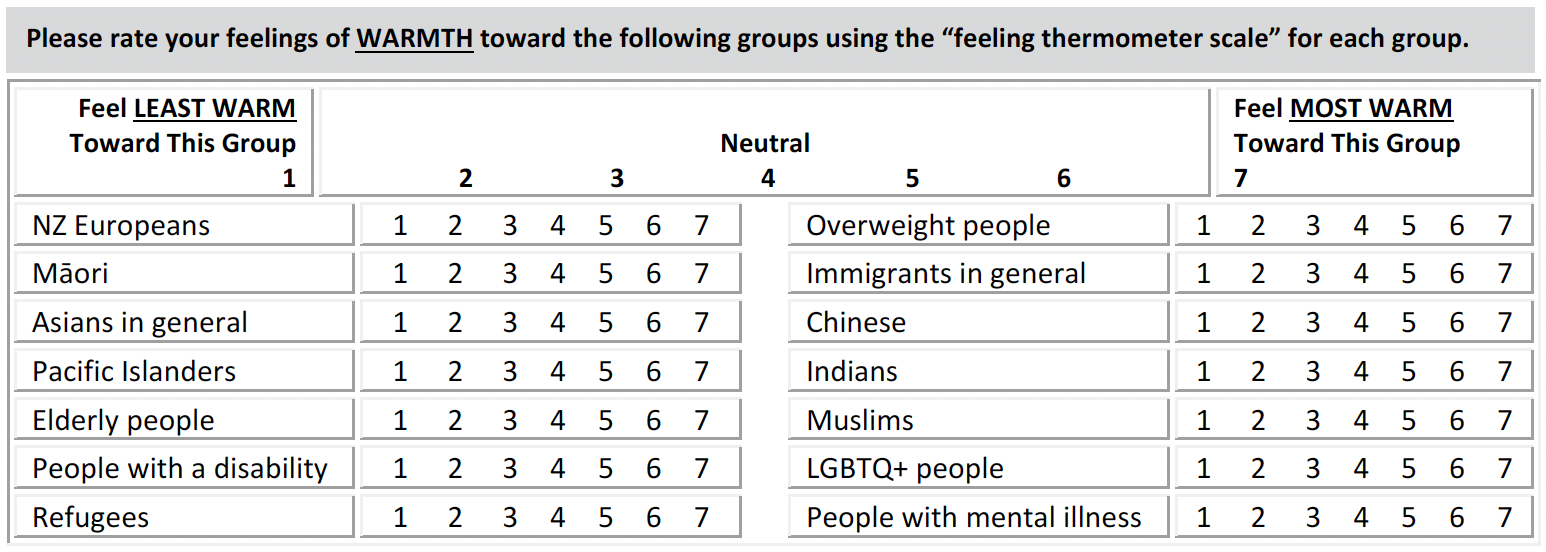
\includegraphics[width=0.75\linewidth,height=\textheight,keepaspectratio]{figs/warmth.png}

}

\caption{\label{fig-warmth}Feeling thermometer scale}

\end{figure}%

\subsubsection{Felt belonging}\label{felt-belonging}

\begin{enumerate}
\def\labelenumi{\arabic{enumi}.}
\tightlist
\item
  I know that people in my life accept and value me. (1 = Very
  Inaccurate, 7 = Very Accurate).
\item
  I feel like an outsider. (1 = Very Inaccurate, 7 = Very Accurate).
\item
  I know that people around me share my attitudes and beliefs. (1 = Very
  Inaccurate, 7 = Very Accurate).
\end{enumerate}

\subsubsection{Support}\label{support}

\begin{enumerate}
\def\labelenumi{\arabic{enumi}.}
\tightlist
\item
  There are people I can depend on to help me if I really need it. (1 =
  Strongly Disagree, 7 = Strongly Agree).
\item
  There is no one I can turn to for guidance in times of stress (R). (1
  = Strongly Disagree, 7 = Strongly Agree).
\item
  I know there are people I can turn to when I need help. (1 = Strongly
  Disagree, 7 = Strongly Agree).
\end{enumerate}

\subsubsection{Employment}\label{employment}

\begin{enumerate}
\def\labelenumi{\arabic{enumi}.}
\tightlist
\item
  What is your highest level of qualification? (String entry).
\item
  Are you currently employed (This includes self-employed or casual
  work)? (Yes/No). This leads to a four-point nominal response: employed
  full-time, employed part-time, unemployed, and not in the labour
  force.
\item
  In that job, what is your current occupation? (String entry).
\item
  What is the main activity of the business or employer that you work
  for? (String entry).
\item
  How long have you worked at your current organization? (String entry:
  years/months).
\item
  How satisfied are you with your current job? (1 = Not Satisfied, 7 =
  Very Satisfied).
\item
  How secure do you feel in your current job? (1 = Not Secure, 7 = Very
  Secure).
\item
  How valued do you feel by your current organization? (1 = Not valued,
  7 = Very Valued).
\end{enumerate}

\subsubsection{Health}\label{health}

\begin{enumerate}
\def\labelenumi{\arabic{enumi}.}
\tightlist
\item
  In general, would you say your health is\ldots{} (1 = Poor, 7 =
  Excellent).
\item
  I seem to get sick a little easier than other people. (1 = Strongly
  Disagree, 7 = Strongly Agree).
\item
  I expect my health to get worse. (1 = Strongly Disagree, 7 = Strongly
  Agree).
\item
  Do you have a health condition or disability that limits you, and that
  has lasted for 6+ months? (Yes/No). If yes, please state: (String
  entry).
\item
  How often do you have a drink containing alcohol? This is measured
  using a 6 point nominal scale (a. Never - I don't drink, b. Monthly or
  less, c.~Up to 4 times a month, d.~Up to 3 times a week, e. 4 or more
  times a week, f.~Don't know).
\item
  Have you ever regularly smoked tobacco cigarettes? (Yes/No).
\item
  Have you ever regularly used e-cigarettes? (Yes/No).
\item
  Do you currently smoke tobacco cigarettes? (Yes/No).
\item
  Do you currently vape or use e-cigarettes? (Yes/No).
\item
  Access to and satisfaction with GP: Do you have a regular family
  doctor/GP? (Yes/No). (If yes) How satisfied are you with the service
  and care you receive from your family doctor/GP? (1 = Not Satisfied, 7
  = Very Satisfied). Do you think your doctor/GP shares a similar
  cultural background to you? (1 = Definitely No, 7 = Definitely Yes).
  Does your doctor/GP respect your cultural background when you are
  discussing health issues with them? (1= Definitely No, 7 = Definitely
  Yes).
\item
  Please estimate how many hours you spent during each of the following
  things last week (String entry). Options provided: Working in paid
  employment, housework/cooking, looking after children,
  volunteer/charitable work, exercising/physical activity, watching
  TV/Netflix/movies, travelling/commuting, watching/reading news, using
  the internet (in total), using social media (e.g., Facebook), playing
  video games/computer games.
\item
  BMI: Calculated by using a person's weight (kg) divided by square root
  of height (m) that is asked separately, using ``What is your height?
  (String entry (metres))'', and ``What is your weight? (String entry
  (kgs))''.
\item
  During the past month, on average, how many hours of actual sleep did
  you get per night? (String entry).
\item
  Do you have a health condition or disability that limits you, and that
  has lasted for 6+ months? (Yes/No). If yes, please state: (String
  entry).
\item
  Chronic diseases diagnosis: See Figure~\ref{fig-chrondis}.
\end{enumerate}

\begin{figure}

\centering{

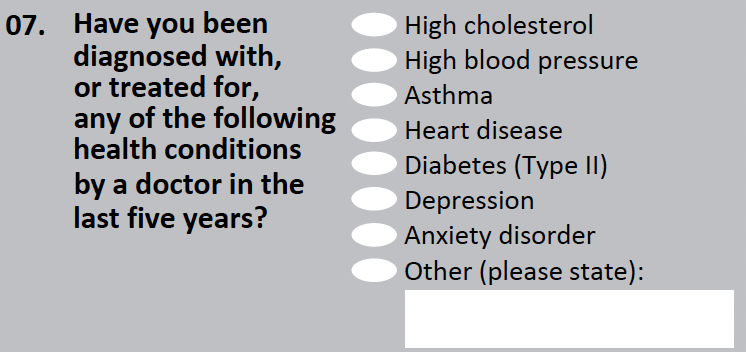
\includegraphics[width=0.75\linewidth,height=\textheight,keepaspectratio]{figs/chronic-disease.png}

}

\caption{\label{fig-chrondis}Chronic disease diagnosis}

\end{figure}%

\subsubsection{Subjective wellbeing/psychological
distress}\label{subjective-wellbeingpsychological-distress}

Measured using the Kessler-6 items (items 1-6 in
Figure~\ref{fig-Kess-6}) rated on a 5-point scale (0 = None of the time,
4 = All of the time) (Kessler et al. 2010).

\begin{figure}

\centering{

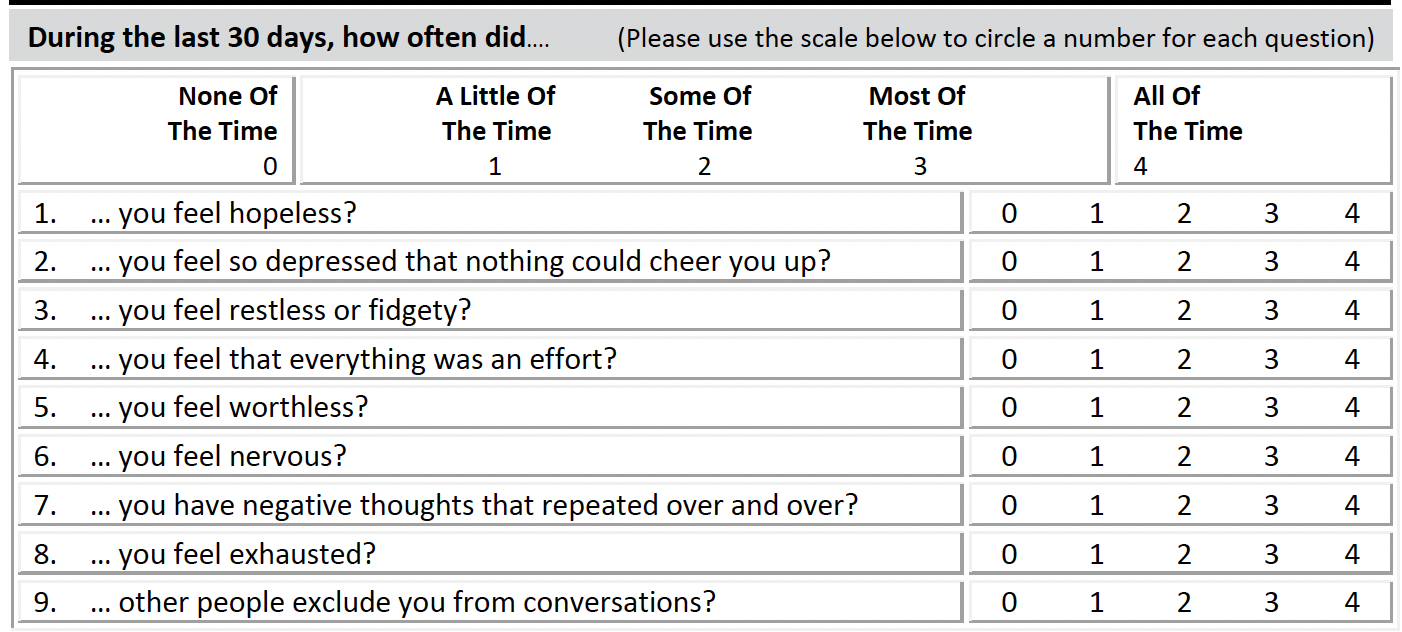
\includegraphics[width=0.75\linewidth,height=\textheight,keepaspectratio]{figs/kessler-6.png}

}

\caption{\label{fig-Kess-6}Kessler-6 subjective wellbeing scale}

\end{figure}%

\subsubsection{Meaning of life}\label{meaning-of-life}

Items are: ``My life has a clear sense of purpose'' (1 = Strongly
Disagree, 7 = Strongly Agree) and ``I have a good sense of what makes my
life meaningful'' (1 = Strongly Disagree, 7 = Strongly Agree).

\subsubsection{Life satisfaction and national
wellbeing}\label{life-satisfaction-and-national-wellbeing}

Items from Figure~\ref{fig-life-sat} measured on 11-item scale (0 =
Completely Dissatisfied, 10 = Completely Satisfied). In addition, ``I am
satisfied with my life (1= Strongly Disagree, 7 = Strongly Agree)'' and
``In most ways my life is close to ideal (1 = Strongly Disagree, 7 =
Strongly Agree)'' are used.

\begin{figure}

\centering{

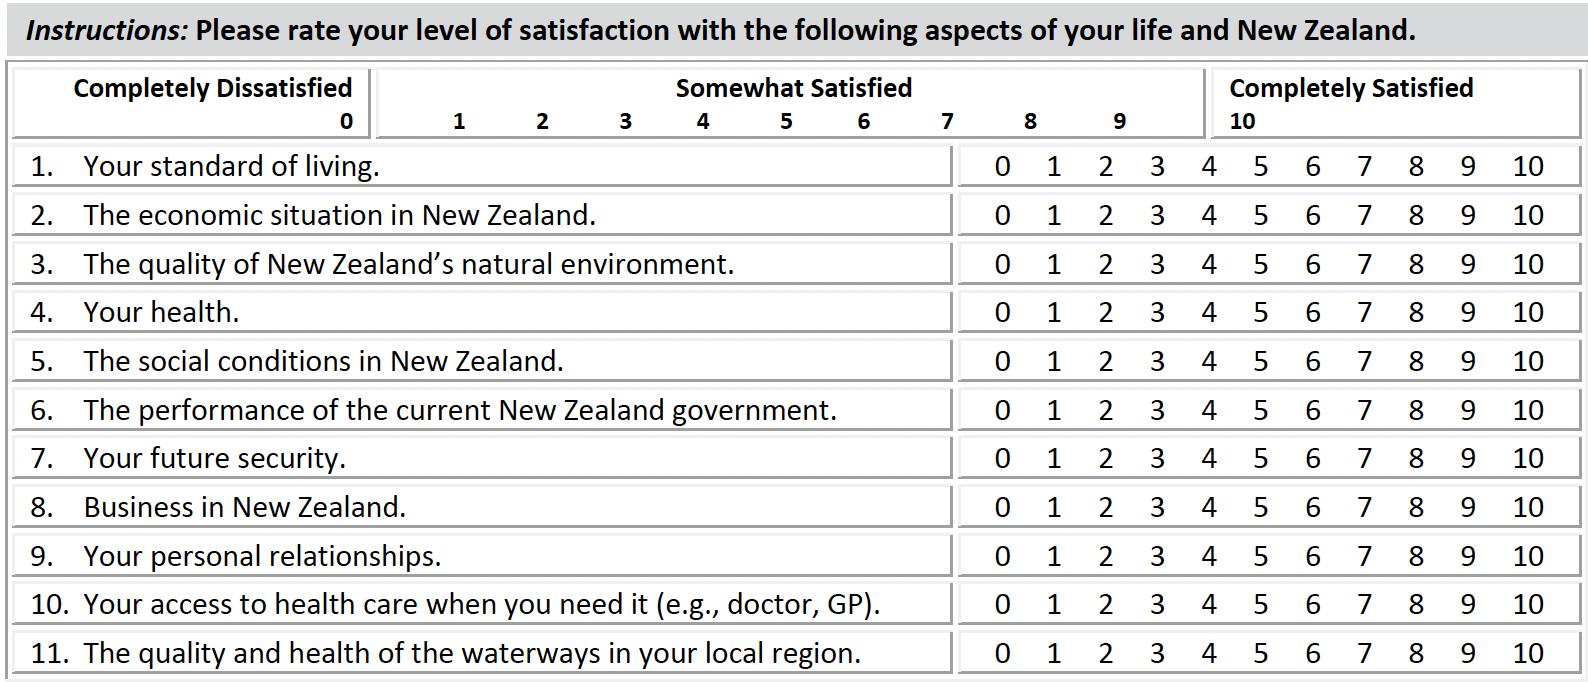
\includegraphics[width=0.75\linewidth,height=\textheight,keepaspectratio]{figs/life-sat.png}

}

\caption{\label{fig-life-sat}Life Satisfaction scale}

\end{figure}%

\subsubsection{Self esteem}\label{self-esteem}

Items are, ``On the whole I am satisfied with myself'' (1 = Very
Inaccurate, 7 = Very Accurate), ``I take a positive attitude toward
myself'' (1 = Very Inaccurate, 7 = Very Accurate) and ``I am inclined to
feel that I am a failure'' (R) (1 = Very Inaccurate, 7 = Very Accurate).

\subsubsection{Gratitude}\label{gratitude}

Items are, ``I have much in my life to be thankful for'' (1 = Strongly
Disagree, 7 = Strongly Agree), ``When I look at the world, I don't see
much to be grateful for'' (R) (1 = Strongly Disagree, 7 = Strongly
Agree) and ``I am grateful to a wide variety of people'' (1 = Strongly
Disagree, 7 = Strongly Agree).

\subsubsection{Community making}\label{community-making}

I feel a sense of community with others in my local neighbourhood (1 =
Strongly Disagree, 7 = Strongly Agree).

\subsubsection{Intergroup anxiety}\label{intergroup-anxiety}

I feel anxious about interacting with people from other races (1 =
Strongly Disagree, 7 = Strongly Agree).

\subsubsection{Rumination}\label{rumination}

During the last 30 days, how often did you have negative thoughts that
repeated over and over? (0 = None of the time, 4 = All of the time).

\subsubsection{Forgivingness versus vengeful
rumination}\label{forgivingness-versus-vengeful-rumination}

Items are, ``Sometimes I can't sleep because of thinking about past
wrongs I have suffered.'' (1 = Strongly Disagree, 7 = Strongly Agree),
``I can usually forgive and forget when someone does me wrong. (R)'' (1
= Strongly Disagree, 7 = Strongly Agree), and ``I find myself regularly
thinking about past times that I have been wronged.'' (1 = Strongly
Disagree, 7 = Strongly Agree).

\subsubsection{Matching with other religious
groups}\label{matching-with-other-religious-groups}

The following demographic variables are measures by which we will
compare the sample obtained with population level indicators of Muslim
Diversity in New Zealand Public records.

\begin{enumerate}
\def\labelenumi{\arabic{enumi}.}
\tightlist
\item
  Age: ``What is your age?'' (String entry), and ``When is your date of
  birth?'' (String entry).
\item
  Education: Measured by an 11-point ordinal scale (0 = No
  Qualification, 11 = Doctoral Degree, based on the New Zealand
  Qualification Framework ({``The New Zealand Qualifications
  Framework''} 2016)) from responses to the qualification-related
  question.
\item
  Employment: A binary variable is created (0 = Unemployed, 1 =
  Employed) based on the responses to the employment item ``Are you
  currently employed?''.
\item
  Ethnicity: The items displayed in Figure~\ref{fig-ethnicgroups} are
  categorised following the New Zealand Census Groups: European, Māori,
  Pacific Peoples, Asian, MELAA (Middle Eastern, Latin
  American/African), and Other.
\item
  Gender: Responses to the string entry item ``What is your gender?''
  will be used to create a binary variable (Male = 1, Not male = 0).
\item
  Area-unit deprivation: Measured based on 2018 New Zealand Deprivation
  Index (Atkinson, Salmond, and Crampton 2019) that assigns a
  decile-rank index (1 = Least Deprived, 10 = Most Deprived) using
  participants' immediate neighbourhood's aggregate census information.
  This index is calculated using component factor analysis of nine
  variables in weighted order as follows: proportion of adults who
  received a means-tested benefit, household income, proportion not
  owning own home, proportion of single-parent families, proportion of
  unemployed, proportion lacking qualifications, proportion of household
  crowding, proportion with no telephone access, and proportion with no
  car access. Hence, this index reflects nationwide mean deprivation
  level for small neighbourhood-type units (i.e., small community areas
  consisting about 80-90 people).
\item
  Socioeconomic status (Occupational prestige): A census-derived
  occupation-based measure NZSEI (New Zealand Socioeconomic Index) is
  used to estimate one's socioeconomic status. It uses an open-ended
  question regarding one's occupation, which is subsequently classified
  in accordance with the Australian and New Zealand Standard
  Classification of Occupations (ANZSCO) Level 3. In case of missing
  values, the measure is imputed using a combination of age and
  education. The measure is assigned scores between 10 = Low and 90 =
  High.
\item
  Parent: Measured by assigning a binary variable (1 = Those with
  children, 0 = The rest) to the item: ``How many children have you
  given birth to, fathered, or adopted?''. (String entry).
\item
  Partner: Responses to ``What is your relationship status?'' are
  assigned a binary variable (1 = Has a partner, 0 = Doesn't have a
  partner).
\item
  Religious identification: Responses to ``Do you identify with a
  religion and/or spiritual group?'' are coded a binary variable (1 =
  Yes, 0 = No).
\item
  Political orientation: Responses to ``Please rate how politically
  left-wing versus right-wing you see yourself as being'' are assigned a
  7-point scale (1 = Extremely left-wing, 7 = Extremely right-wing).
\item
  Residence: Urban or rural residence (a two-item nominal variable) is
  identified based on the physical addresses provided.
\item
  Region of habituation: Whether participants are living in an urban or
  rural area, based on the addresses provided, is coded 1 = Urban, 0 =
  Rural.
\item
  Race-based rejection anxiety: ``People from other races would be
  likely to reject me on the basis of my race''. (1 = Strongly Disagree,
  7 = Strongly Agree).
\item
  Big Six personality traits: Six personality traits -- agreeableness,
  conscientiousness, extraversion, openness, honesty-humility, and
  neuroticism -- are measured using a 7-point (1 = Very Inaccurate, 7 =
  Very Accurate) Mini-IPIP6 scale (Sibley et al. 2011).
\end{enumerate}

\begin{figure}

\centering{

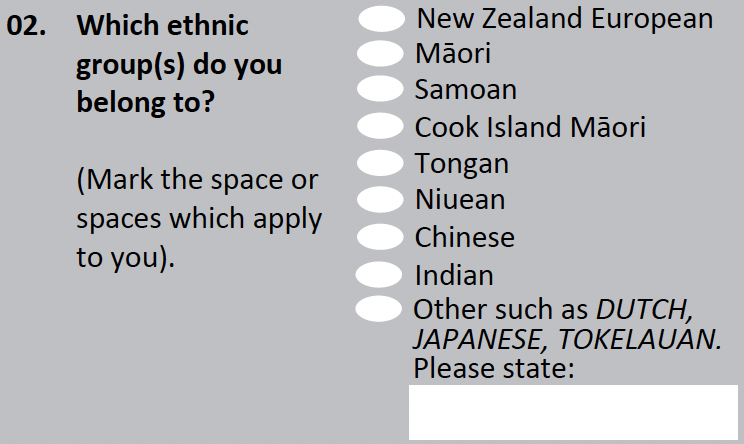
\includegraphics[width=0.75\linewidth,height=\textheight,keepaspectratio]{figs/ethnic-groups.png}

}

\caption{\label{fig-ethnicgroups}Ethnic groups}

\end{figure}%

\subsection{Ethics}\label{ethics}

The NZAVS was approved by the University of Auckland Human Participants
Ethics Committee on 26 May 2021 until 26 May 2027 (Reference:
UAHPEC22576). All participants granted informed written consent and the
University of Auckland Human Participants Ethics Committee approved all
procedures.

\subsection{Design}\label{design}

The NZAVS is a comprehensive, planned 20-year longitudinal national
probability panel study that began in 2009, focusing on social
attitudes, personality, ideology, and health outcomes of adults in New
Zealand. Currently in its 16th wave, the NZAVS employs quantitative
measures to gather data from adult New Zealanders. The MDS serves as a
booster to the NZAVS, specifically aimed at increasing the participation
of Muslims residing in New Zealand. The MDS Wave 1 corresponded to NZAVS
Wave 15 (from October 15, 2023, to October 14, 2024). Subsequent waves
of the MDS align with NZAVS Wave 16 (October 15, 2024, to October 14,
2025), Wave 17 (October 15, 2025, to October 14, 2026), and so on. MDS
will examine various outcome variables to test the proposed hypotheses,
including perceived religious and ethnic discrimination, employment
status, job satisfaction, job security, feeling valued by the
organisation, self-rated health, perceived health decline, chronic
diseases and disabilities, psychological distress, meaning of life, life
satisfaction, sense of belonging, perceived support, warmth toward
various groups, vengeful rumination, and forgivingness. The predictors
variables include:

\begin{enumerate}
\def\labelenumi{\arabic{enumi}.}
\tightlist
\item
  Perceived religious discrimination
\item
  Perceived ethnic discrimination
\item
  Employment status
\item
  Job satisfaction
\item
  Job security
\item
  Feeling valued by organisation
\item
  Self-rated health
\item
  Perceived health decline
\item
  Chronic diseases and disabilities
\item
  Kessler-6 psychological distress scale
\item
  Meaning of life
\item
  Life satisfaction
\item
  Sense of belonging
\item
  Perceived support
\item
  Warmth toward various groups
\item
  Vengeful rumination
\item
  Forgivingness
\end{enumerate}

\subsection{Research questions}\label{research-questions}

\begin{enumerate}
\def\labelenumi{\arabic{enumi}.}
\tightlist
\item
  Do service attendance and/or prayer practices buffer Muslims against
  experiences of anti-Muslim prejudice?
\item
  What is the relationship between community ties and resilience to
  anti-Muslim prejudice among Muslims?
\item
  Do Muslims face more challenges in employment compared to members of
  other religious groups?
\item
  How do health outcomes for Muslims differ from those of matched
  members of other religious groups?
\item
  How does religious community-making influence subjective well-being,
  meaning in life, and psychological distress among Muslims? And, in
  what ways do these outcomes compare between Muslims and matched
  members of other religious groups?
\end{enumerate}

\subsection{Procedure}\label{procedure}

\subsubsection{Training, Support, and Supervision for the Project
Team}\label{training-support-and-supervision-for-the-project-team}

The research assistant position was advertised by the University of
Canterbury and shared via social media, emails, and community
organisations. The eligibility criteria included at least tertiary level
education in New Zealand, familiarity with research in humanities and
social sciences, interest in working with communities, and experiences
of working with Muslim community organisations. Thirty research
assistants, as detailed in Table~\ref{tbl-muslim-population}, were
recruited after initial screening and interviews from a total of 95
applicants.

Prior to the commencement of the MDS, a series of comprehensive Zoom
training sessions were conducted to equip the research assistants with
the necessary knowledge and skills. These sessions covered the
background of the NZAVS and the MDS, as well as detailed instructions on
the survey questionnaires. Additionally, the training emphasised ethical
guidelines, confidentiality principles, and effective communication
strategies for engaging with a culturally diverse participant pool. The
training also provided guidelines on planning for hiring participants
and promoting community participation in the study. All recommendations
from the co-designing process with the community were included in the
training material.

The training programme was tailored to accommodate varying levels of
research experience. For some assistants, this was their first
experience in data collection, while others had extensive research
backgrounds. This structured support system ensured that research
assistants were well-prepared and confident in their roles, contributing
to the overall success of the project.

\subsubsection{Data collection}\label{data-collection}

Research assistants used the snowball approach for data collection. As
per recommendations from the co-designing process, they started reaching
out to their primary contacts first. These consisted of family members
and close friends that the research assistants found the most
comfortable to reach out to. Starting in this manner ensured that the
research assistants were put in a real-life situation within their
comfort zone. MUA provided them with consistent feedback and was
available to help those that needed practice communicating the message.

After two weeks, the research assistants were guided to reach out to
their secondary contacts. These consisted of extended families, peers,
and classmates. The process of feedback and support by MUA continued.
Finally, they reached out to community organisations. This gradual
extension helped research assistants to build confidence in reaching out
and attain coherence of narrative regarding the study. Research
assistants with extensive previous engagement experience with the
community reached out to the community sooner than the rest. In addition
to promotion, the research assistants were available to help
participants with understanding questions, and if needed, were also
present when participants completed questionnaires.

The sample was non-representative, and participants had the choice of
filling in the online questionnaire using Qualtrics, or a paper
questionnaire which could be returned to the NZAVS headquarters in
Auckland University using a prepaid postal envelope.

A runsheet was provided, and different documents and promotional
materials such as individual messages, community messages, flyers, and
posters were at the research assistants disposal based on their needs.
We also developed vision and ethics statements that were part of our MDS
introductory letter. In addition, a cover letter was sent to all
participants alongside the information sheet. It was aimed to clearly
convey the purposes of MDS to the community, see appendices A-H for the
aforementioned materials. Furthermore, 10 promotional shirts were
designed which the research assistants wore during festivals and
community events for the study promotion.

The social media campaign started at the beginning of 2024 and continued
until the end of Wave 1. Besides regularly posting on a weekly, and
later on, a fortnightly basis, we also used paid promotion to increase
the reach of the project.

For the purposes of community promotion, we relied on a combination of
community outreach at local mosques, religious, community, and ethnic
organisations, Muslim schools and businesses, and MSAs (Muslim Student
Associations). From available databases and community contacts, we
identified 218 organisations and the research assistants were able to
approach Muslims in 105 of these organisations. Out of these, 80
endorsed and promoted the study. Different organisations endorsed us in
different manners: some allowed us to give speeches to their audience,
while others shared our promotional material online on their social
media platforms, via community message groups (e.g., WhatsApp), and
mailing lists. It is worth noting that some of these organisations did
not necessarily belong to the Muslim community (e.g., refugee
resettlement centres and ethnic community trusts), though they still
offered support. In addition, tens of posters were placed in community
facilities (e.g., mosques and libraries) and hundreds of flyers were
handed over after Friday prayers as well as cultural, community, and
religious events and festivals.

In addition to reaching out to organisations, the principal investigator
and research assistants conversed with 28 local and national community
leaders, celebrities, religious scholars, and academics to disseminate
information about the study to the communities. As part of this
recruitment drive, the principal investigator, MUA, also presented 28
talks, presentations, and/or lectures to Muslim community groups around
New Zealand via mosques, universities and community organisations in the
selected cities, explaining the goals of the NZAVS, and how it would
benefit the New Zealand Muslim community to be represented in this
ongoing national longitudinal panel sample. Five additional talks were
delivered by the research assistants too.

\subsubsection{Ensuring research assistants'
convenience}\label{ensuring-research-assistants-convenience}

MDS research assistants came from varied backgrounds. Some of them have
had research degrees and extensive research experience, whereas, for
others, it was their first attempt at engaging in data collection. Some
research assistants wanted explicit weekly targets while others decided
their own targets. The principal investigator, MUA, also provided
ongoing guidance and feedback, and was available to communicate with
participants via audio and video mediums if and when needed. MUA
conducted fortnightly check-ins with the research assistants and teams
in each selected city to ensure that all their queries were answered,
and that they had reliable guidance and feedback throughout the process.

\subsubsection{Web hosting}\label{web-hosting}

The MDS website (access from
\href{https://linktr.ee/muslimdiversity}{here}) provides all key
information for the public and will be updated as progress is made.

\subsubsection{Data management}\label{data-management}

The collected data were anonymised and processed in the NZAVS
headquarters, and only made available to trusted researchers and
collaborators. The NZAVS data dictionary, sampling procedure, sample
details and other relevant information can be accessed online
(\url{https://osf.io/75snb/wiki/home/}) (Sibley 2024).

\subsection{Timeline}\label{timeline}

\begin{figure}

\centering{

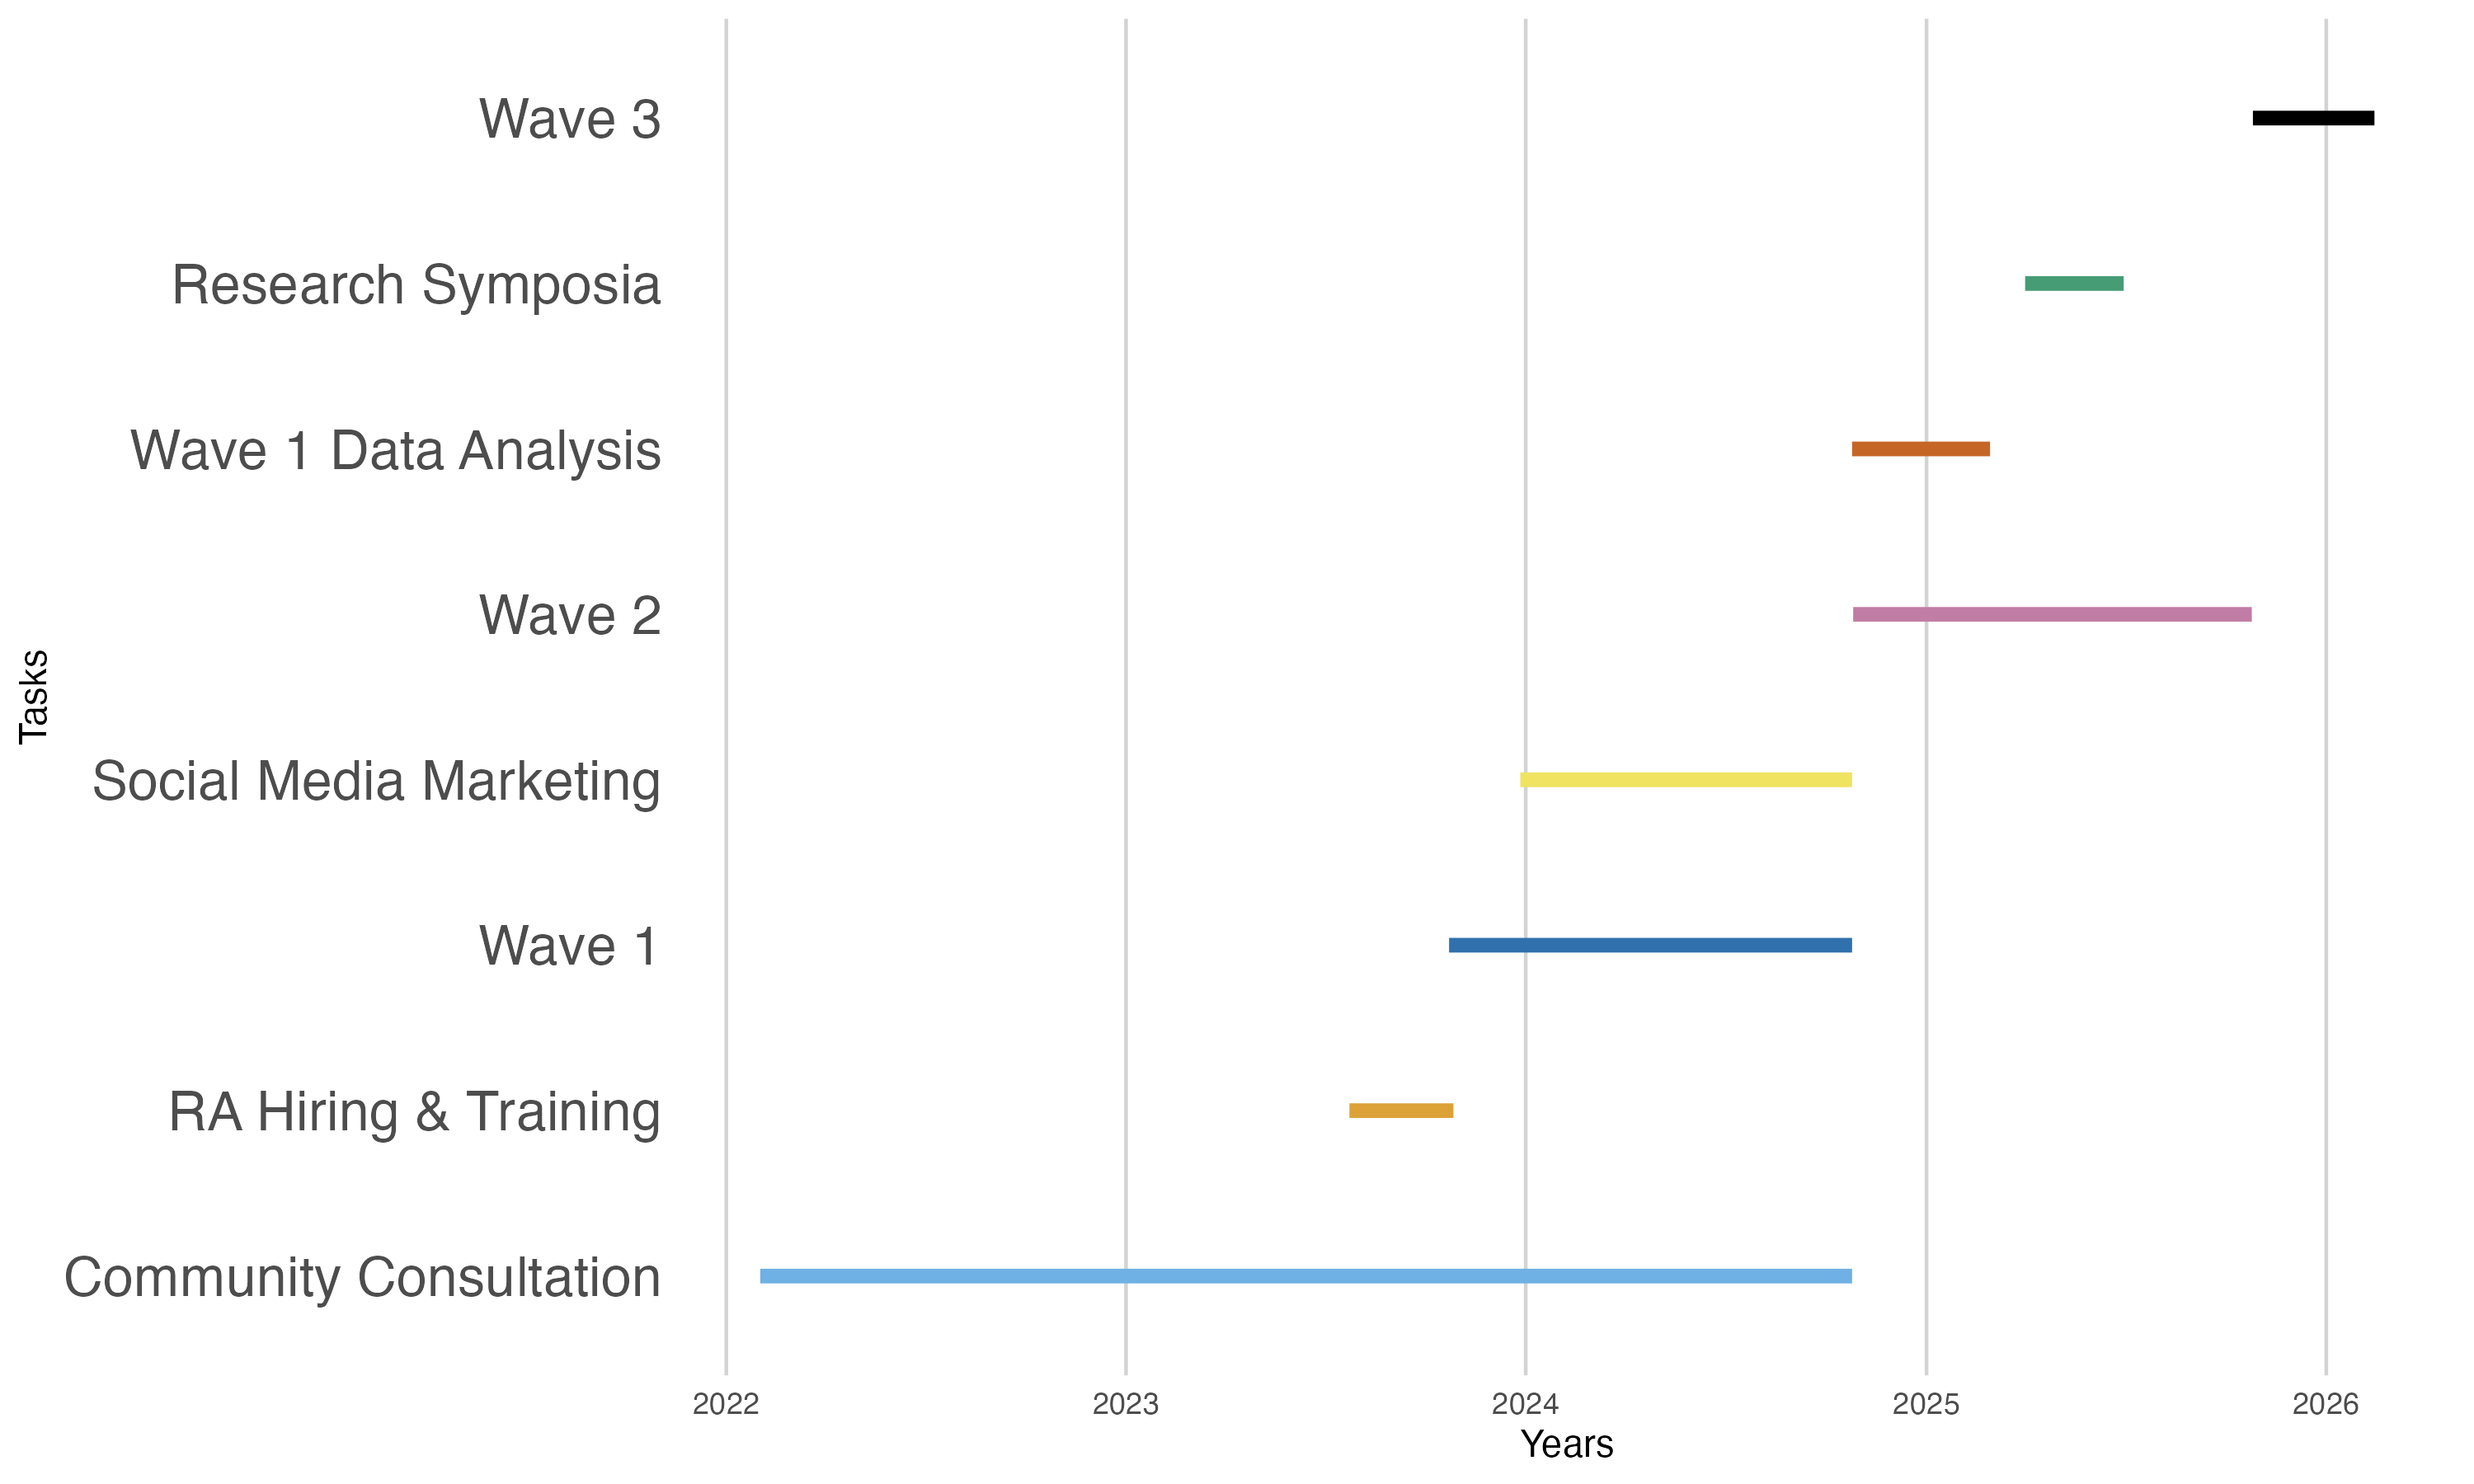
\includegraphics[width=1\linewidth,height=\textheight,keepaspectratio]{figs/project_timeline.png}

}

\caption{\label{fig-timeline}MDS timeline showing tasks and durations}

\end{figure}%

As displayed in Figure~\ref{fig-timeline}, the community consultation
started before Wave 1 and continued until the end of it. In addition,
social media marketing has been an integral part of MDS data collection
campaigns. The planned future events, with approximate dates, are
indicated too.

\section{Part 3: Lessons learned - Guidelines for working with the
Muslim
community}\label{part-3-lessons-learned---guidelines-for-working-with-the-muslim-community}

Based on our interactions with the community, we had anecdotal evidence
that some members of the Muslim community might distrust social science
research and view it as state surveillance. We also had anecdotal
evidence of increases in such scepticism after the Christchurch
shootings. Hence, we ensured that our approach and methodology addressed
these issues beforehand, and in-line with recommendations from
co-designing with the community, such as building trust, highlighting
the importance and benefits of academic research, and addressing
under-representation of Mulsims in research. Our flyers, posters, social
media messages, and individual messages are testaments to this. Based on
our interactions with the Muslim community and feedback from the
research assistants, we inferred that the following elements encourage
increased participation of the Muslim community in research:

\begin{enumerate}
\def\labelenumi{\arabic{enumi}.}
\item
  Building rapport: The community trusts religious and community
  leaders, intellectuals, academics, and elderly. The first step in any
  community interaction would be reaching out to such figures and
  clearly sharing with them the vision, mission, and need for the
  project. Leaders' endorsement can be extremely influential.
\item
  Addressing concerns regarding confidentiality and data management:
  Given that a large number of Muslims have taken refuge in New Zealand
  after escaping oppressive regimes, it is only natural for them to be
  sceptical of anyone who might ask for data. Therefore, it is extremely
  important to ensure that the data are secured. At NZAVS, we adhere to
  strict security protocols. Our data are anonymised yet not publicly
  available, and is safeguarded with some of the world's most secure
  encryption.
\item
  Being transparent and truthful with the community: Besides building
  rapport and ensuring confidentiality, it is extremely important to be
  transparent and truthful with the community in terms of deliverables
  and outputs. Reportedly, in the past, some researchers have collected
  data from the community, but the reports were not shared. Being in
  constant contact with the community ensures that future research
  endeavours could take place effectively.
\item
  Reaching out to individuals personally, and not via groups: Our
  research assistants have discovered this, especially by the means of
  targeting their close circles individually and keeping expanding the
  reach, as a more effective approach to incur higher response rate as
  compared to targeting the community via organisations.
  Notwithstanding, the group approach has its own advantages and helps
  with dissemination of messages.
\item
  Medium: At the beginning, the focus was on both online and paper
  questionnaires. Towards the end, based on the feedback from research
  assistants, we employed paper questionnaires only, which resulted in a
  comparatively higher response rate.
\item
  Achievable targets: After testing different targets, each research
  assistant committed to the completion of a minimum of three
  participants each week during the final five months. This, coupled
  with point 5, enhanced the response rate.
\item
  Comprehensive promotion and research assistant training and support:
  We found the use of social media, website, flyers, and posters
  effective in engaging the community. Contents of the website
  addressing privacy concerns, ethics, vision, and mission were
  appreciated by some participants and community leaders. In terms of
  research assistant training, we learned that a systematic approach,
  runsheet, manual, frequently asked questions, and evolving data
  collection targets were useful.
\end{enumerate}

Similarly, we learned that the following factors could hinder data
collection efforts.

\begin{enumerate}
\def\labelenumi{\arabic{enumi}.}
\tightlist
\item
  Length of the questionnaire: It is measured by the time taken to
  complete the questionnaire, and was one of the challenges identified
  in MDS. This would not necessarily generalise to shorter
  questionnaires.
\item
  Unfamiliarity of participants with scientific research: Generally, it
  is the subsequent generation of Muslims that attend the Western
  education system and become familiar with the process of research,
  thereby, being more comfortable with research participation. On the
  other hand, the first generations are less likely to participate. We
  also have anecdotal evidence from participants, research assistants,
  and Advisory Group to infer that the first generation of Muslims, due
  to language barriers and other life priorities (settling in New
  Zealand, work, lower education) might be less likely to participate.
  Therefore, the sampling should be mindful of these barriers and
  implement appropriate recruitment strategies.
\item
  Privacy concerns: In general, if the community does not trust the
  research group, they would be hesitant to participate. It might sound
  like common sense, but this is an alert for researchers to not take
  this matter lightly. The community might not be very familiar with the
  research process, but that does not mean they should be approached in
  a non-serious or frank manner. All the potential concerns, including
  privacy, have to be addressed beforehand.
\item
  Political climate: The current political climate and the Middle-East
  conflict have affected the population as well as the research
  assistants. Although we lack empirical data, many of our team members
  and potential participants lost their loved ones since October 2023
  and have been grieving. In some of such instances, we tried not to
  approach affected members of the community.
\item
  Language barriers: Our community consultation revealed that most of
  our potential participants would comprehend English. This, by design,
  left out those with limited language abilities from participation.
\end{enumerate}

We witnessed enhanced participation by addressing these challenges. Some
of these recommendations have been reflected in outputs of the March 15
research group too (Sulaiman-Hill, Porter, et al. 2024).

\subsection{Strengths of MDS}\label{strengths-of-mds}

MDS represents a significant advancement in knowledge production,
addressing the historical under-representation of the Muslim community
in research. While the NZAVS has made important contributions in this
area, MDS is a crucial step forward.

As the first comprehensive, contextually rich study of Kiwi Muslims, MDS
uses systematic, standardized research methods to explore the
decision-making, policy formulation, and inclusion practices of key
social players such as the news media, political parties, and social
action groups. By ensuring a representative sample (with the NZAVS
comprising more than 1\% of the target population), MDS aims to enhance
our understanding of how these entities interact with the Muslim
community in New Zealand.

The findings of MDS are expected to provide valuable insights into
issues like political perceptions, diversity, discrimination,
self-perception, resilience, meaning-making, and flourishing within the
Muslim community. Additionally, MDS will help dispel misconceptions and
improve the general public's understanding of Muslims, fostering greater
social cohesion. Furthermore, this research lays a solid foundation for
future studies on the experiences and perspectives of Muslims in New
Zealand.

\subsection{Limitations of MDS design}\label{limitations-of-mds-design}

MDS is a quantitative-only study, which was necessary to enable
comparison with other groups in the NZAVS and to serve as a booster for
the NZAS. While this focus on quantitative data limits certain aspects
of the study, it provides valuable insights and lays the groundwork for
future qualitative research, which could address emerging questions from
the community. Given the large sample size and the range of variables
examining various social aspects, MDS---and the NZAVS more
broadly---offers an unprecedented wealth of data about the lives of New
Zealanders. This richness is demonstrated by 300+ peer-reviewed
publications that have emerged from the datasets.

A limitation of the study is its focus on English-speaking participants,
which may restrict the generalisability of the findings. This approach
was necessary for ensuring comparability with other groups in the NZAVS,
but a future qualitative follow-up study could aim to include
non-English speakers and further broaden the scope of the research.

Another challenge was the length of the questionnaire, which may have
affected overall participation and completion rates. However, gathering
detailed data on these variables was deemed essential for enhancing the
NZAVS dataset and making meaningful comparisons across religious groups.

Finally, because MDS follows the same structure as the NZAVS, some
survey items may not be fully culturally compatible with the attitudes
and beliefs of the Muslim community. However, feedback from the Advisory
Group indicated that these items did not need to be removed, as they
were considered important for the overall study framework.

\subsection{Application and implications of MDS
findings}\label{application-and-implications-of-mds-findings}

This research enables Muslims in New Zealand to be active participants
in shaping their unique identity. This identity not only encapsulates
the diverse ethnocultural societies within the New Zealand Muslim
community, but also allows for the formation of a distinct national
identity. Often research used to drive policy and intervention targeted
at New Zealand Muslims is informed by research undertaken on Muslim
communities overseas. Whilst there are many comparable similarities
between Muslims worldwide, their everyday life experiences are heavily
shaped by the society in which a Muslim resides. Furthermore, the
strengthening of this identity can facilitate greater in-group
understanding, connection, and belonging to New Zealand.

This research also has the potential for the Muslim voice to have a
greater influence on public perception of Muslims in New Zealand. The
visible Muslim voice in many parts of the Western world is often
reactionary to political events, discriminatory experiences, or
accusations of terror. Greater understanding and public discourse of
lived experiences of Muslims in New Zealand, one allows for a more
accurate understanding of these experiences, and two, facilitates a
shift in how Muslim voices are `allowed' to participate in society.

This research can also inform international discourse on the experiences
of Muslim immigrants, and their views and beliefs on their country of
residence. Stockemer and Moreau (2021) completed a comprehensive review
on studies focused on Muslim immigrants' sense of belonging and
identity; results reflected this varied greatly depending on the country
of residence at a macro-level, and personal education at the
micro-level.

MDS allows Muslim to have an active, data informed input in shaping
policies and intervention targeted at their wellbeing and livelihood.
This is especially significant in the aftermath of the 15 March terror
attacks targeting Muslims in New Zealand. Research highlights
significant long term mental health distress and vulnerability for
individuals directly impacted by the attacks (Sulaiman-Hill, Schluter,
et al. 2024).

Insights from the findings could be used as a form of policy advocacy in
two ways: first, by engaging with policymakers to advocate for policies
that address discrimination and promote inclusivity. This could involve
working with local governments and organisations to ensure that the
voices of Muslims are heard in policymaking and in organising safety and
security initiatives. Second, by collaborating with law enforcement to
create safety initiatives that ensure the wellbeing of Muslim
communities.

Policymakers can use our findings to develop more effective and
equitable policies that better address the needs and rights of Muslim
communities. For instance, understanding the impact of community ties
and religiosity on the resilience of Muslim communities can guide the
government in creating support programmes that strengthen these aspects.

Findings from this study can contribute to government strategies that
focus on adaptability and change while engaging with the Muslim
community to encourage bonding, bridging, and linking social capital
where possible.

Research also highlights the psychological impact that the terror
attacks had on wider Muslim communities in New Zealand, who viewed the
attack to be of a personal nature through a shared identity with the
targeted victims of the attacks (Nasier 2023). This poses significant
responsibility on the health system in New Zealand to be equipped to
meet the ongoing and long-term needs of New Zealanders impacted by
terror. This research can provide valuable insights into the Muslim
community, facilitating the development of interventions that are
effectively tailored to meet their needs.

Practically, the findings could guide the development of targeted
interventions aimed at reducing Islamophobia and supporting the Muslim
community in New Zealand. Since ``programmes are the instruments,
governments use to implement a policy or achieve a particular outcome''
(Rose 1991), community-based programmes that strengthen social ties and
religious practices could be designed to buffer against anti-Muslim
prejudice. Insights from the findings could further pave the way for
organising public forums and discussions to bring together Muslims and
non-Muslims to address issues of discrimination, resilience, and
community wellbeing, with the aim of fostering dialogue and
understanding.

The findings could also inform policy regarding the need for targeted
anti-discrimination measures. As the research has highlighted the
challenges faced by Muslims in employment and health, targeted
interventions to improve these areas for Muslim communities should be
prioritised by the government. Muslims in New Zealand are diverse and
the Muslim community organisations have been actively working with local
and central governments to provide advice and input regarding ethnic
communities ({``Federation of Islamic Associations of New Zealand''}
2024; {``New Zealand Muslim Association''} 2024). However, it should be
noted that while it may be regarded as illusory to develop policies,
programmes, and practices that purport to be ``blind'' to race and
ethnicity (Durie 2005), socio-economic measures addressing
discrimination among Muslims in New Zealand should be tailored to the
communities, considering their religious characteristics alongside their
ethnicities or races.

Regarding socio-economic concerns, the practical applications of the
study's findings can be seen in interventions focusing on employment and
economic support, such as creating programmes that assist Muslims in
navigating the job market and addressing the unique challenges they
face. This could include mentorship programmes, skills training, and
networking opportunities. Additionally, partnerships between local
businesses and Muslim community organisations could promote diversity in
hiring practices and support entrepreneurs. Culturally sensitive mental
health initiatives that are visible within Muslim communities and
tailored to their cultural and religious needs would also be effective
programmes.

\subsection{Conclusion}\label{conclusion}

MDS is a crucial booster for the NZAVS because not only it addresses the
under-representation of Muslim in NZAVS, but it only helps us answer
many questions about Muslims' self-perception, meaning-making,
flourishing, religiosity, and health outcomes. We have provided a
preliminary guideline of working with a minoritised religious community
in a culturally sensitive manner. Despite the well-known limitations of
observational, quantitative, survey research, MDS provides substantial
values in terms of implications and applications. Techniques learned
from MDS can be applied while working with Muslims and other culturally
similar groups in New Zealand and overseas.

\newpage{}

\section*{References}\label{references}
\addcontentsline{toc}{section}{References}

\phantomsection\label{refs}
\begin{CSLReferences}{1}{0}
\bibitem[\citeproctext]{ref-religi2024}
{``2023 {C}ensus {P}opulation, {D}welling, and {H}ousing
{H}ighlights.''} 2024.
\url{https://www.stats.govt.nz/information-releases/2023-census-population-dwelling-and-housing-highlights/}.

\bibitem[\citeproctext]{ref-arkilic2020}
Arkilic, Ayca. 2020. {``What Is {I}slam's Appeal to {M}{ā}ori?''}
\url{http://newsroom.co.nz/2020/08/18/what-is-islams-appeal-to-maori/}.

\bibitem[\citeproctext]{ref-arkilic2021a}
---------. 2021. {``The {C}hristchurch Shooting and the 2020 {N}ew
{Z}ealand Election.''} In, edited by Stephen Levine, 225--39.
Wellington, New Zealand: Victoria University Press.

\bibitem[\citeproctext]{ref-atkinson2019}
Atkinson, June, Clare Salmond, and Peter Crampton. 2019. {``NZDep2018
Index of Deprivation.''}

\bibitem[\citeproctext]{ref-bulbulia2023}
Bulbulia, Joseph A, M Usman Afzali, Kumar Yogeeswaran, and Chris G
Sibley. 2023. {``Long-Term Causal Effects of Far-Right Terrorism in New
Zealand.''} Edited by M Gelfand. \emph{PNAS Nexus} 2 (8).
\url{https://doi.org/10.1093/pnasnexus/pgad242}.

\bibitem[\citeproctext]{ref-byrne2022}
Byrne, Kate G., Kumar Yogeeswaran, Martin J. Dorahy, Jessica Gale, M.
Usman Afzali, Joseph Bulbulia, and Chris G. Sibley. 2022.
{``Psychological Impact of Far-Right Terrorism Against Muslim Minorities
on National Distress, Community, and Wellbeing.''} \emph{Scientific
Reports} 12 (1): 1620. \url{https://doi.org/10.1038/s41598-022-05678-x}.

\bibitem[\citeproctext]{ref-drury2016}
Drury, A. 2016. {``{Islam{'}s} History and Integration in the {N}ew
{Z}ealand Society: A {convert{'}s} View.''} In, edited by E Kolig and
Voyce M, 113--29. Maryland, USA: Rowman.

\bibitem[\citeproctext]{ref-durie2005}
Durie, Mason. 2005. {``Race and Ethnicity in Public Policy: Does It
Work?''} \emph{Social Policy Journal of New Zealand Te Puna Whakaaro}
24: 1--11.
\url{https://www.msd.govt.nz/about-msd-and-our-work/publications-resources/journals-and-magazines/social-policy-journal/spj24/24-race-and-ethnicity-in-public-policydoes-it-work-p1-11.html}.

\bibitem[\citeproctext]{ref-fianz2024}
{``Federation of Islamic Associations of New Zealand.''} 2024.
\url{https://fianz.com/general-advocacy/}.

\bibitem[\citeproctext]{ref-frykberg2023}
Frykberg, Laura. 2023. {``Online Hate Towards Muslims 'Increasing' Since
Mosque Attacks.''}
\url{https://www.1news.co.nz/2023/03/12/online-hate-towards-muslims-increasing-since-mosque-attacks/}.

\bibitem[\citeproctext]{ref-greaves2020}
Greaves, Lara M., Aarif Rasheed, Stephanie D'Souza, Nichola Shackleton,
Luke D. Oldfield, Chris G. Sibley, Barry Milne, and Joseph Bulbulia.
2020. {``Comparative Study of Attitudes to Religious Groups in New
Zealand Reveals Muslim-Specific Prejudice.''} \emph{K{ō}tuitui: New
Zealand Journal of Social Sciences Online} 15 (2): 260--79.
\url{https://doi.org/10.1080/1177083x.2020.1733032}.

\bibitem[\citeproctext]{ref-greenfield2019}
Greenfield, Charlotte. 2019. {``Lives Forever Changed by Christchurch
Shootings.''} \emph{Reuters}.
\url{https://widerimage.reuters.com/story/lives-forever-changed-by-christchurch-shootings}.

\bibitem[\citeproctext]{ref-hawi2019}
Hawi, Diala, Danny Osborne, Joseph Bulbulia, and Chris G. Sibley. 2019.
{``Terrorism Anxiety and Attitudes Toward Muslims.''} \emph{New Zealand
Journal of Psychology} 48 (1): 8089.

\bibitem[\citeproctext]{ref-islamoph2022}
{``Islamophobia After {C}hristchurch Terror Attacks Quadrupled -
{A}ustralian Report.''} 2022.
\url{https://www.rnz.co.nz/news/national/463304/islamophobia-after-christchurch-terror-attacks-quadrupled-australian-report}.

\bibitem[\citeproctext]{ref-jacinda2019b}
{``Jacinda {A}rdern on the {C}hristchurch Shooting: {`}One of {N}ew
{Z}ealand's Darkest Days'.''} 2019.
\url{https://www.theguardian.com/world/2019/mar/15/one-of-new-zealands-darkest-days-jacinda-ardern-responds-to-christchurch-shooting}.

\bibitem[\citeproctext]{ref-junaid2024}
Junaid, Fatima A., S. Cassim, and J. Khan-Janif. 2024. {``Muslims'
Experiences of Inclusion, Discrimination, {I}slamophobia and Wellbeing
in {A}otearoa {N}ew {Z}ealand.''}
\url{https://doi.org/10.13140/RG.2.2.12693.74725/1}.

\bibitem[\citeproctext]{ref-kabir2024}
Kabir, Shah Nister. 2024. {``{`}They Are Us{'}: Orientalist Perspective
Challenged in New Zealand Newspapers{'} Coverage.''} \emph{Journal of
Arab \& Muslim Media Research}, January.
\url{https://doi.org/10.1386/jammr_00077_1}.

\bibitem[\citeproctext]{ref-kessler2010}
Kessler, Ronald C., Jennifer Greif Green, Michael J. Gruber, Nancy A.
Sampson, Evelyn Bromet, Marius Cuitan, Toshi A. Furukawa, et al. 2010.
{``Screening for Serious Mental Illness in the General Population with
the K6 Screening Scale: Results from the WHO World Mental Health (WMH)
Survey Initiative.''} \emph{International Journal of Methods in
Psychiatric Research} 19 (S1): 4--22.
\url{https://doi.org/10.1002/mpr.310}.

\bibitem[\citeproctext]{ref-nasier2023}
Nasier, B A. 2023. {``{`This Is {U}s'}: {Y}oung {N}ew {Z}ealand
{M}uslims' Responses to the {M}arch 15th {T}errorist {A}ttacks in
{C}hristchurch.''} PhD thesis, Auckland.

\bibitem[\citeproctext]{ref-nzma2024}
{``New Zealand Muslim Association.''} 2024.
\url{https://www.ethniccommunities.govt.nz/community-directory/show/1170}.

\bibitem[\citeproctext]{ref-oliver2024}
Oliver, Katie. 2024. {``Survivor Who Lost His Wife in Christchurch
Terror Attack Shares His Love for Forgiveness.''} \emph{Newshub}.
\url{https://www.newshub.co.nz/home/new-zealand/2024/03/survivor-farid-ahmed-who-lost-his-wife-in-christchurch-terror-attack-shares-his-love-for-forgiveness.html}.

\bibitem[\citeproctext]{ref-rahman2019}
Rahman, Anjum. 2019. {``Islamic {W}omen's {C}ouncil Repeatedly Lobbied
to Stem Discrimination.''}
\url{https://www.rnz.co.nz/news/on-the-inside/384911/islamic-women-s-council-repeatedly-lobbied-to-stem-discrimination}.

\bibitem[\citeproctext]{ref-rahman2020}
Rahman, Khairiah A. 2020. {``News Media and the Muslim Identity After
the Christchurch Mosque Massacres.''} \emph{K{ō}tuitui: New Zealand
Journal of Social Sciences Online} 15 (2): 360--84.
\url{https://doi.org/10.1080/1177083x.2020.1747503}.

\bibitem[\citeproctext]{ref-raissi2024}
Raissi, Hussain. 2024. {``Exploring Senses of Belonging: {A}
Multidimensional Study of {M}uslim Immigrant Youth in {N}ew
{Z}ealand.''} PhD thesis, Dunedin.

\bibitem[\citeproctext]{ref-rose1991}
Rose, Richard. 1991. {``What Is Lesson-Drawing?''} \emph{Journal of
Public Policy} 11 (1): 3--30.
\url{https://doi.org/10.1017/s0143814x00004918}.

\bibitem[\citeproctext]{ref-royalco2020}
{``Royal {C}ommission of {I}nquiry into the Terrorist Attack on
{C}hristchurch {M}asjidain on 15 {M}arch 2019.''} 2020.
\url{https://christchurchattack.royalcommission.nz}.

\bibitem[\citeproctext]{ref-shanaah2021}
Shanaah, Sadi, Kumar Yogeeswaran, Lara Greaves, Joseph A. Bulbulia,
Danny Osborne, M. Usman Afzali, and Chris G. Sibley. 2021. {``Hate
Begets Warmth? The Impact of an Anti-{M}uslim Terrorist Attack on Public
Attitudes Toward {M}uslims.''} \emph{Terrorism and Political Violence},
119.

\bibitem[\citeproctext]{ref-shaver2017}
Shaver, John H., Chris G. Sibley, Danny Osborne, and Joseph Bulbulia.
2017. {``News Exposure Predicts Anti-Muslim Prejudice.''} Edited by
Michiel van Elk. \emph{PLoS One} 12 (3): e0174606.
\url{https://doi.org/10.1371/journal.pone.0174606}.

\bibitem[\citeproctext]{ref-shaver2016}
Shaver, John H., Geoffrey Troughton, Chris G. Sibley, and Joseph A.
Bulbulia. 2016. {``Religion and the Unmaking of Prejudice Toward
Muslims: Evidence from a Large National Sample.''} Edited by Michiel van
Elk. \emph{PLoS One} 11 (3): e0150209.
\url{https://doi.org/10.1371/journal.pone.0150209}.

\bibitem[\citeproctext]{ref-sibley2024}
Sibley, Chris G. 2024. {``New Zealand Attitudes and Values Study.''}
\url{https://osf.io/75snb/wiki/home/}.

\bibitem[\citeproctext]{ref-sibley2020}
Sibley, Chris G., M. Usman Afzali, Nicole Satherley, Anastasia Ejova,
Samantha Stronge, Kumar Yogeeswaran, Michael Grimshaw, Diala Hawi, Zahra
Mirnajafi, and Fiona Kate Barlow. 2020. {``Prejudice Toward {M}uslims in
{N}ew {Z}ealand: Insights from the {N}ew {Z}ealand {A}ttitudes and
{V}alues {S}tudy.''} \emph{New Zealand Journal of Psychology} 49 (1).

\bibitem[\citeproctext]{ref-sibley2011}
Sibley, Chris G., N. Luyten, Missy Purnomo, A. Mobberley, L. W. Wootton,
Matthew Hammond, Nikhil Sengupta, et al. 2011. {``The Mini-IPIP6:
Validation and Extension of a Short Measure of the {B}ig-{S}ix Factors
of Personality in {N}ew {Z}ealand.''} \emph{New Zealand Journal of
Psychology} 40 (3): 142--59.

\bibitem[\citeproctext]{ref-statsnz2024}
{``Stats NZ.''} 2024. \url{https://www.stats.govt.nz/}.

\bibitem[\citeproctext]{ref-stockemer2021}
Stockemer, Daniel, and Shona Moreau. 2021. {``Muslim Immigrants' Sense
of Identity and Belonging in the Western World: A Comprehensive
Review.''} \emph{Nations and Nationalism} 27 (1): 223--37.
\url{https://doi.org/10.1111/nana.12691}.

\bibitem[\citeproctext]{ref-sulaiman-hill2024}
Sulaiman-Hill, Ruqayya C., Richard Porter, Philip Schluter, Ben
Beaglehole, Shaystah Dean, Sandila Tanveer, Joseph Boden, and Caroline
Bell. 2024. {``Research Following Trauma in Minority Ethnic and Faith
Communities: Lessons from a Study of the Psychosocial Sequelae of the
Christchurch Mosque Terror Attacks.''} \emph{BJPsych Open} 10 (1).
\url{https://doi.org/10.1192/bjo.2023.641}.

\bibitem[\citeproctext]{ref-sulaiman-hill2021}
Sulaiman-Hill, Ruqayya C., Richard Porter, Sandila Tanveer, Joseph
Boden, Ben Beaglehole, Philip J. Schluter, Shaystah Dean, and Caroline
Bell. 2021. {``Psychosocial Impacts on the {C}hristchurch {M}uslim
Community Following the 15 March Terrorist Attacks: A Mixed-Methods
Study Protocol.''} \emph{BMJ Open} 11 (10): e055413.

\bibitem[\citeproctext]{ref-sulaiman-hill2024a}
Sulaiman-Hill, Ruqayya C., Philip J Schluter, Sandila Tanveer, Joseph M
Boden, Richard Porter, Ben Beaglehole, Shaystah Dean, Zimna Thaufeeg,
and Caroline Bell. 2024. {``The Psychosocial Impacts of the 15 March
Terrorist Attack on the Christchurch Muslim Community: A Descriptive,
Cross-Sectional Assessment.''} \emph{Australian \& New Zealand Journal
of Psychiatry} 58 (11): 977--89.
\url{https://doi.org/10.1177/00048674241276802}.

\bibitem[\citeproctext]{ref-thenew2016}
{``The New Zealand Qualifications Framework.''} 2016.

\bibitem[\citeproctext]{ref-vanderweele2017}
VanderWeele, Tyler J. 2017a. {``On the Promotion of Human
Flourishing.''} \emph{Proceedings of the National Academy of Sciences}
114 (31): 8148--56. \url{https://doi.org/10.1073/pnas.1702996114}.

\bibitem[\citeproctext]{ref-vanderweele2017a}
---------. 2017b. {``Religious Communities and Human Flourishing.''}
\emph{Current Directions in Psychological Science} 26 (5): 476--81.
\url{https://doi.org/10.1177/0963721417721526}.

\bibitem[\citeproctext]{ref-wilson2020}
Wilson, Chris, and Sanjal Shastri. 2020. {``Hate Crimes Against
{M}uslims Spiked After the Mosque Attacks, and {A}rdern Promises to Make
Such Abuse Illegal.''}
\url{http://theconversation.com/hate-crimes-against-muslims-spiked-after-the-mosque-attacks-and-ardern-promises-to-make-such-abuse-illegal-147347}.

\bibitem[\citeproctext]{ref-worldle2019}
{``World Leaders Condemn New Zealand Mosque Attacks.''} 2019.
\url{https://www.aljazeera.com/news/2019/3/15/the-world-reacts-to-new-zealand-mosque-attacks}.

\bibitem[\citeproctext]{ref-yogeeswaran2019}
Yogeeswaran, Kumar, M Usman Afzali, Nadia P Andrews, Elizabeth A
Chivers, Meng-Jie Wang, Thierry Devos, and Chris G Sibley. 2019.
{``Exploring {N}ew {Z}ealand National Identity and Its Importance for
Attitudes Toward {M}uslims and Support for Diversity.''} \emph{New
Zealand Journal of Psychology} 48 (1): 29--35.

\end{CSLReferences}

\newpage{}

\section{Data Sharing}\label{data-sharing}

The data described in this study are part of the Muslim Diversity Study,
which is conducted under the \href{https://osf.io/75snb/}{New Zealand
Attitudes and Values Study}.

\newpage{}

\section{Conflict of Interest}\label{conflict-of-interest}

The authors have no conflicts of interest to disclose.

\newpage{}

\section{Funding}\label{funding}

The Muslim Diversity Study - officially known as ``A National
Longitudinal Study of Muslim Diversity and Flourishing'' is supported by
a grant from the Templeton Religion Trust (TRT-2022-30579). The funders
had no role in preparing the manuscript or the decision to publish it.

\newpage{}

\section{Acknowledgement}\label{acknowledgement}

The authors are grateful to Michael Mahoney for the
\href{https://github.com/mikemahoney218/quarto-tandf}{Quarto template}.

\newpage{}

\section{Author Roles (CRediT
Taxonomy)}\label{author-roles-credit-taxonomy}

\textbf{M. Usman Afzali:} Conceptualization, Data Curation, Formal
Analysis, Funding Acquisition, Investigation, Methodology, Project
Administration, Resources, Supervision, Visualization, Writing -
Original Draft, Writing - Review \& Editing.

\textbf{Jamila S. Badis:} Project Administration, Writing - Original
Draft, Writing - Review \& Editing.

\textbf{Parus Khoso:} Formal Analysis, Investigation, Writing - Original
Draft.

\textbf{Gul e Aqsa:} Investigation, Writing - Original Draft.

\textbf{Mazharuddin Syed Ahmed:} Writing - Original Draft.

\textbf{Aamina Ali:} Writing - Original Draft.

\textbf{Afrah Ali:} Writing - Review \& Editing.

\textbf{Zarqa Shaheen Ali:} Investigation, Writing - Original Draft.

\textbf{Ayca Arkilic:} Writing - Original Draft, Writing - Review \&
Editing.

\textbf{Tuba Azeem:} Investigation, Writing - Original Draft.

\textbf{Hala Burhoum:} Investigation, Writing - Original Draft.

\textbf{Zahra Emamzadeh:} Writing - Original Draft.

\textbf{Zahra Haidary:} Investigation, Writing - Original Draft.

\textbf{Nasratullah Hamid:} Investigation, Writing - Original Draft.

\textbf{Iman Husain:} Investigation, Writing - Original Draft.

\textbf{Fatima A. Junaid:} Writing - Original Draft, Writing - Review \&
Editing.

\textbf{Mashal Khan:} Investigation, Writing - Original Draft.

\textbf{Adepate Mustapha-Koiki:} Writing - Original Draft.

\textbf{Hussain Raissi:} Investigation, Writing - Original Draft.

\textbf{Farah Shawkat:} Investigation, Writing - Original Draft.

\textbf{Rizwan Sulehry:} Writing - Original Draft.

\textbf{Mai Tamimi:} Investigation, Writing - Original Draft.

\textbf{Sandila Tanveer:} Writing - Review \& Editing.

\textbf{Somia Tasneem:} Writing - Original Draft.

\textbf{Kumar Yogeeswaran:} Conceptualization, Funding Acquisition,
Methodology, Supervision, Writing - Original Draft, Writing - Review \&
Editing.

\textbf{Chris G. Sibley:} Conceptualization, Data Curation, Funding
Acquisition, Methodology, Project Administration, Resources,
Supervision, Writing - Review \& Editing, Development \& Management of
the New Zealand Attitudes and Values Study Panel Data Collection from
2009 to the Present.

\textbf{Joseph A. Bulbulia:} Conceptualization, Funding Acquisition,
Methodology, Project Administration, Resources, Supervision, Writing -
Original Draft, Writing - Review \& Editing.

\textbf{Aarif A. Rasheed:} Conceptualization, Funding Acquisition,
Resources, Writing - Review \& Editing.

\newpage{}

\section{Appendix A: MDS Runhseet}\label{appendix-a-mds-runhseet}

{[}\texttt{Monospaced} font refers to urls in the actual document.{]}

\noindent Salam alaikum and welcome to the Muslim Diversity Study.

\begin{enumerate}
\def\labelenumi{\arabic{enumi}.}
\tightlist
\item
  This \texttt{Dropbox\ folder} consists of all information that you
  might need.
\item
  We have updated our communication and approach strategy, found
  \texttt{here}.
\item
  This \texttt{document} contains message to the community and FAQs.
  {[}will keep updating{]}
\item
  \texttt{Cover\ letter} for the Muslim Diversity Study.
\item
  MDS \texttt{Questionnaire} (pdf)
\item
  Use this \texttt{message} to send the MDS participation request to
  individuals. Please remember that individual connection is extremely
  important, and this is what we bank on.
\item
  Use this \texttt{message} to advertise MDS on social media (e.g.,
  Facebook or LinkedIn); and to send it via WhatsApp or emailing lists
  to the wider community and organisations.
\item
  Use this \texttt{message} for shorter social media platforms (e.g.,
  Twitter/X).
\item
  Access the \texttt{poster} (pdf) here (and png).
\item
  Access the \texttt{flyer} (pdf) here (and png).
\item
  This \texttt{document} can be shared with organisations to introduce
  MDS.
\item
  Organisation lists: \texttt{Auckland}, \texttt{Hamilton},
  \texttt{Palmerston\ North}, \texttt{Wellington},
  \texttt{Christchurch}, \texttt{Dunedin}. In addition, \texttt{this} is
  the list of organisations that have endorsed us or shared our ads.
  Please keep adding names to this list.
\item
  Please use \texttt{this} guideline for reaching out to organisations.
\item
  This \texttt{story} by UC has recorded the motivation behind MDS and
  its benefits for the Muslim community. It can be shared widely with
  those that want to know more.
\item
  The recent public \texttt{lecture} narrates the whole story of MDS
  (past, present, future) in a detailed manner. This, again, can be
  shared extensively with anyone interested.
\item
  Find our social media and website \texttt{here}.
\item
  The paper questionnaires are valuable, and to ensure meaningful
  responses, we shall only provide them to individuals who express
  interest and want them. Please distribute as many copies of
  \texttt{flyers}, and I can provide more flyers as needed.
\item
  Participants using the Qualtrics link should be reminded that they can
  resume the questionnaire from where they left off if they don't
  complete it initially. Ideally, an additional message can be sent
  using this wording: ``You can easily resume the questionnaire where
  you left off by clicking on the provided link. Feel free to complete
  the questionnaire in multiple sessions; your previous responses are
  automatically saved.'' Since it's not part of the ethics approval, it
  can be sent in the next message as additional guideline (instruction).
\item
  To claim your hours, log-in \texttt{here}.
\item
  If you are claiming your hours for the first time, use information in
  this \texttt{folder}.
\item
  If you want to have an update on collected data so far, see
  \texttt{this}.
\item
  I am thinking of a qualitative research project based on our
  experiences with the Muslim community where we'd want to interview our
  current RA's. It's briefly detailed \texttt{here}. If any of you are
  keen to be part of this or know someone who might want to take this
  on, please let me know. It can easily be a master's thesis, and as
  detailed in the brief, it will attract great impact.
\item
  \url{https://linktr.ee/muslims_nz}
\item
  \url{https://linktr.ee/muslimdiversity}
\end{enumerate}

\newpage{}

\section{Appendix B: Message to Individual
Participants}\label{appendix-b-message-to-individual-participants}

Your Voice Matters! Join the Muslim Diversity Study!

\noindent Assalamu Alaikum WR WB {[}person's name{]}

\noindent I'm {[}name of the RA{]}, a research assistant in the Muslim
Diversity Study.

\noindent We need YOUR perspective!

\noindent The Muslim community is underrepresented, and we're changing
that with your help. Participate in this first-of-its-kind survey to
share your views on social attitudes, values, resilience, religiosity,
flourishing, meaning-making, wellbeing, and experiences of Muslims in
New Zealand. Let's make our voices heard!

\noindent Why Participate?

\noindent Gather data on underrepresented Muslims, amplifying voices and
providing insights into issues, wellbeing, and experiences.

\noindent Equip the Muslim community with evidence-based information for
advocacy.

\noindent Enrich understanding, strengthening the collective voice, and
shaping a more accurate narrative.

\noindent Your contribution counts and confidentially is assured!

\noindent By participating, you could potentially win one out of five
\$1000 grocery vouchers.

\noindent The data will be analysed with a focus on the Muslim
community. Your input guides our research, ensuring authenticity and
representation. We reassure you that the responses to the questionnaire
are anonymized, encrypted, and aggregated in a manner that ensure
confidentiality.

\noindent Spread the Word!

\noindent Please share with your friends, family, and community members!
Let's come together and make a difference.

\noindent To complete the questionnaire kindly click on the link below
or message us for a paper copy:
\url{https://www.nzavs.auckland.ac.nz/muslim_diversity}

\noindent For more info, visit our website (below) or reach out to Dr
Usman Afzali (the lead researcher): (email address and contact phone
number)
\url{https://www.canterbury.ac.nz/science/schools/psyc-speech-hear/research/muslim-diversity/}

\noindent APPROVED BY THE UNIVERSITY OF AUCKLAND HUMAN PARTICIPANTS
ETHICS COMMITTEE ON 26/05/2021 UNTIL 26/05/2027, REFERENCE NUMBER:
UAHPEC22576.

\newpage{}

\section{Appendix C: Community and Social Media
Message}\label{appendix-c-community-and-social-media-message}

Your Voice Matters! Join the Muslim Diversity Study!

\noindent Assalamu Alaikum WR WB, Muslims in New Zealand!

\noindent We need YOUR perspective!

\noindent The Muslim community is underrepresented, and we're changing
that with your help. Participate in this first-of-its-kind survey to
share your views on social attitudes, values, resilience, religiosity,
flourishing, meaning-making, wellbeing, and experiences of Muslims in
New Zealand. Let's make our voices heard!

\noindent Why Participate?

\noindent Gather data on underrepresented Muslims, amplifying voices and
providing insights into issues, wellbeing, and experiences.

\noindent Equip the Muslim community with evidence-based information for
advocacy.

\noindent Enrich understanding, strengthening the collective voice, and
shaping a more accurate narrative.

\noindent Your contribution counts and confidentially is assured!

\noindent By participating, you could potentially win one out of five
\$1000 grocery vouchers.

\noindent The data will be analysed with a focus on the Muslim
community. Your input guides our research, ensuring authenticity and
representation. We reassure you that the responses to the questionnaire
are anonymized, encrypted, and aggregated in a manner that ensure
confidentiality.

\noindent Spread the Word!

\noindent Please share with your friends, family, and community members!
Let's come together and make a difference.

\noindent To complete the questionnaire kindly click on the link below
or message us for a paper copy:
\url{https://www.nzavs.auckland.ac.nz/muslim_diversity}

\noindent For more info, visit our website (below) or reach out to Dr
Usman Afzali (the lead researcher): (email address and contact phone
number)
\url{https://www.canterbury.ac.nz/science/schools/psyc-speech-hear/research/muslim-diversity/}

\noindent APPROVED BY THE UNIVERSITY OF AUCKLAND HUMAN PARTICIPANTS
ETHICS COMMITTEE ON 26/05/2021 UNTIL 26/05/2027, REFERENCE NUMBER:
UAHPEC22576.

\newpage{}

\section{Appendix D: MDS Flyer}\label{appendix-d-mds-flyer}

\begin{figure}

\centering{

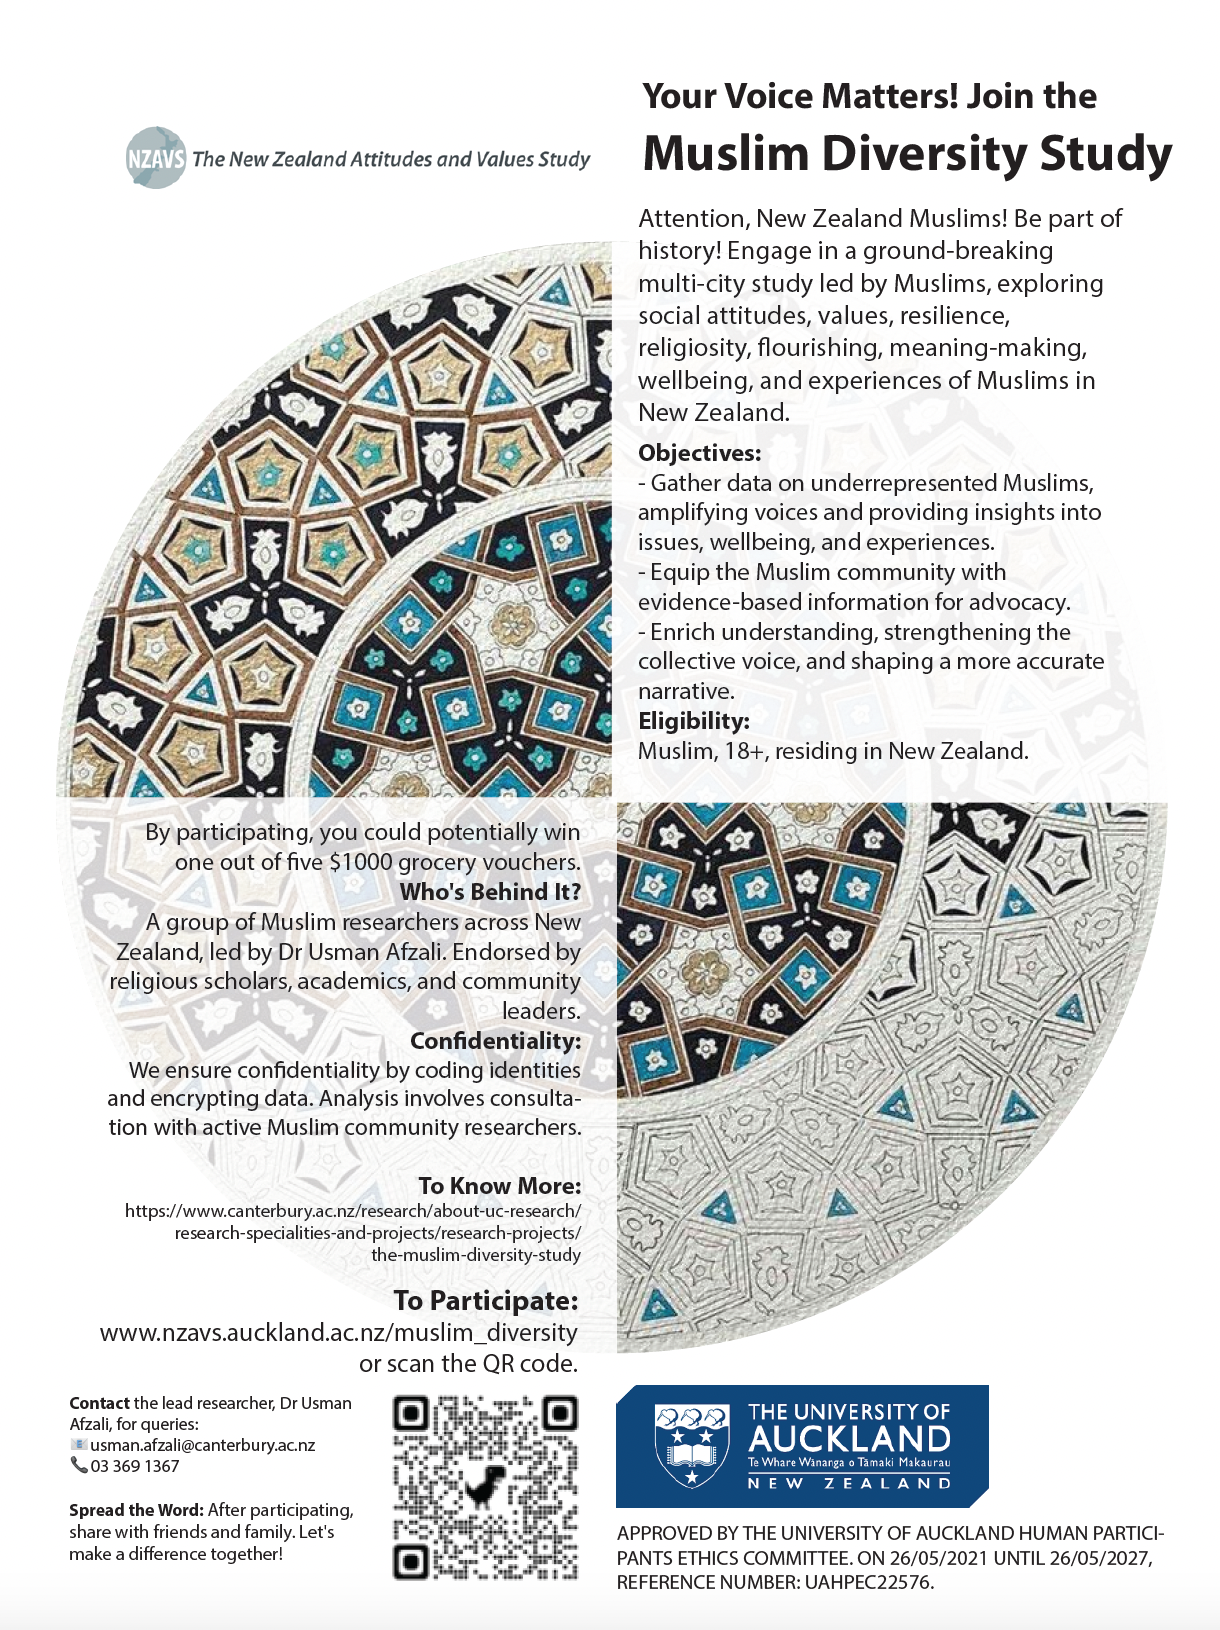
\includegraphics[width=0.8\linewidth,height=\textheight,keepaspectratio]{figs/flyer-v1.png}

}

\caption{\label{fig-appendfig}MDS Flyer}

\end{figure}%

\newpage{}

\section{Appendix E: MDS Poster}\label{appendix-e-mds-poster}

\begin{figure}

\centering{

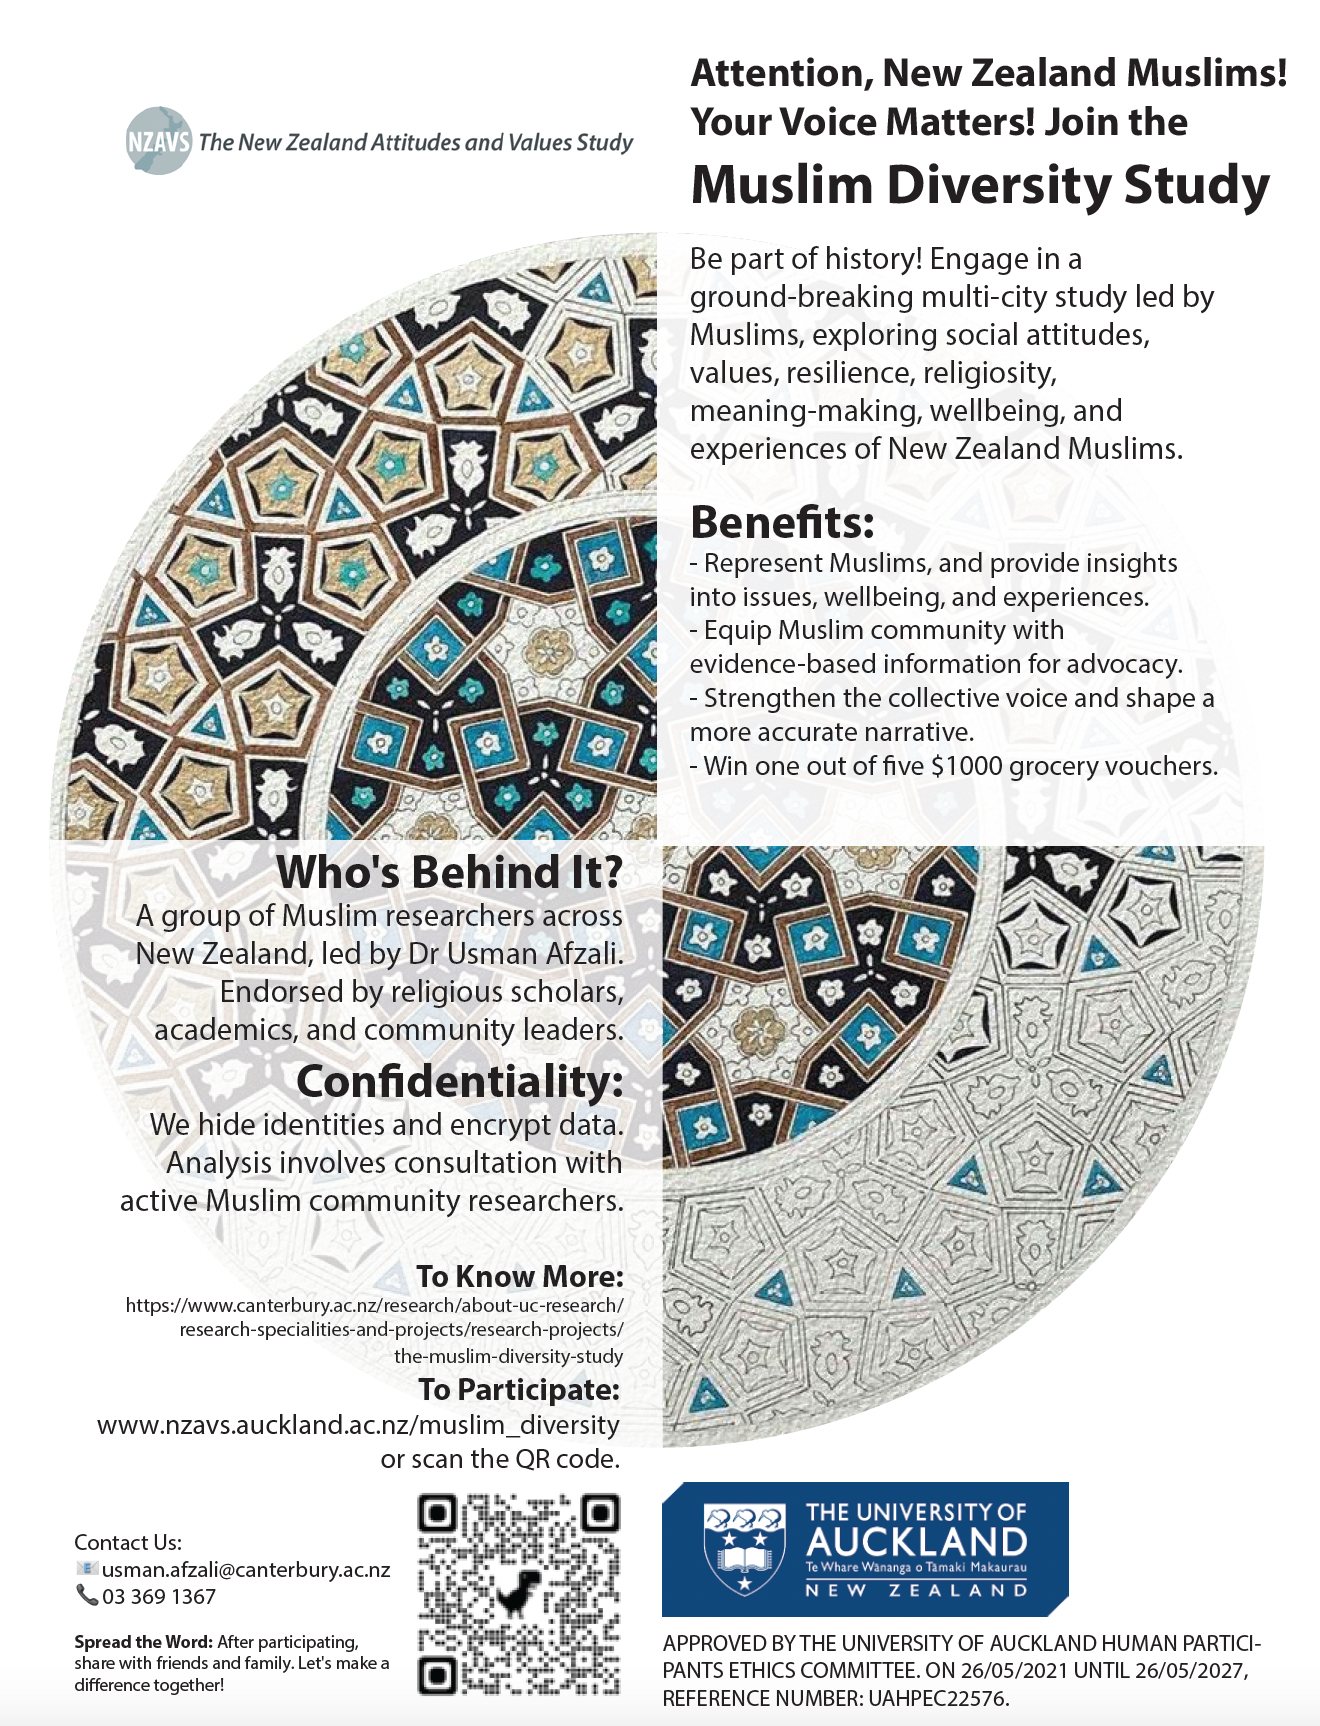
\includegraphics[width=0.8\linewidth,height=\textheight,keepaspectratio]{figs/poster-v1.png}

}

\caption{\label{fig-appendfig1}MDS Poster}

\end{figure}%

\newpage{}

\section{Appendix F: MDS Vision}\label{appendix-f-mds-vision}

The NZAVS is committed to the following three principles for the Muslim
Diversity Study.

\noindent Protection: The NZAVS is strongly committed to respecting and
protecting data gathered from all participants and takes confidentiality
seriously. Our commitment to participant privacy and safety is central
to the NZAVS.

\noindent Participation: The NZAVS is committed to enhancing the
research capacity of our communities in Aotearoa New Zealand. Any NZAVS
research focusing specifically on the Muslim community will be reviewed
by our Muslim academic advisor Dr Usman Afzali, and/or appropriate
nominated reviewers from the Muslim community in New Zealand. We are
committed to Muslim community-led research for Muslim-focussed studies
to ensure respectful reporting that considers the social, religious, and
cultural settings of New Zealand's Muslims.

\noindent Partnership: The NZAVS actively fosters opportunities for
collaborative research with emerging Muslim researchers in New Zealand.
We seek to mentor Muslim graduate students interested in accessing NZAVS
data for research in their own postgraduate theses or dissertations. We
invite students from the Muslim community in New Zealand to contact our
Muslim academic advisor, or any member of the NZAVS board or leadership
team for guidance in developing a project.

\newpage{}

\section{Appendix G}\label{appendix-g}

\subsection{Participant
confidentiality}\label{participant-confidentiality}

\noindent Here at the NZAVS we take our participants' confidentiality
very seriously. All personal details are encrypted and stored separately
from questionnaire data. Only Professor Chris Sibley and trusted
research assistants working on the NZAVS in secure conditions have
access to participants' contact details. Participants' contact details
are used solely for the purposes of contacting them to continue their
participation in the NZAVS each year and to provide them with
information and feedback about research findings from the NZAVS.

\noindent Reference: \url{https://osf.io/75snb/wiki/home/}

\subsection{Ethics approval}\label{ethics-approval}

\noindent The Muslim Diversity Study is regulated by the University of
Auckland Human Participants Ethics Committee.

\noindent The current ethics approval statement for the 2021-2027 period
is as follows: The New Zealand Attitudes and Values Study was approved
by the University of Auckland Human Participants Ethics Committee on
26/05/2021 until 26/05/2024, and renewed on 02/05/2023 until 26/05/2027.
Reference Number: UAHPEC22576.

\noindent For any queries regarding ethical concerns, you may contact
the Chair, University of Auckland Human Participants Ethics Committee,
Ethics and Integrity Team, University of Auckland, Private Bag 92019,
Auckland 1142. Telephone 09 373-7599 ext. 83711. Email:
\href{mailto:humanethics@auckland.ac.nz}{\nolinkurl{humanethics@auckland.ac.nz}}.

\subsection{Why we need ethics
approval?}\label{why-we-need-ethics-approval}

\noindent Ethical approval for research is essential to ensure that
studies involving human participants are conducted in a morally
responsible and respectful manner. It serves to protect the rights,
wellbeing, dignity, and confidentiality of those involved in the
research, as well as the broader community affected by the study.
Ethical approval ensures that potential risks are minimized, benefits
are maximized, informed consent is obtained, and any potential conflicts
of interest or biases are addressed. This oversight helps maintain
public trust in the scientific community and upholds the fundamental
principles of fairness, respect, and accountability in research
endeavours.

\newpage{}

\section{Appendix H: MDS Cover
Letter}\label{appendix-h-mds-cover-letter}

\noindent Salaam alaikum, kia ora, and greetings!

\noindent My name is Dr Usman Afzali, and I am the lead researcher of
the Muslim Diversity Study. The Muslim Diversity Study is conducted as
part of the New Zealand Attitudes and Values Study. This is a broad
longitudinal study aiming to survey people from all across New Zealand
(see the information sheet on the next page for more details).

\noindent As a researcher and committed member of the New Zealand Muslim
community, I recognise the importance of including our voices in
discussions about New Zealand. This inspired me to develop a booster
study to enhance Muslim representation in the New Zealand Attitudes and
Values Study, since we are underrepresented at present. I would be
deeply grateful if you would consider participating in this survey. By
sharing your perspectives, you will enrich our understanding of the
attitudes, values, and wellbeing of the Muslim community in New Zealand.
This will strengthen the voice of our community within New Zealand. We
will publish the findings of our work in scientific journals, create
brief reports and infographics, and present our findings to Muslim
communities across New Zealand over the coming years.

\noindent My research team includes Muslim researchers from across New
Zealand. By completing this survey, you are contributing to a research
project led by people from the Muslim community for the Muslim community
in New Zealand. Furthermore, analysis of the collected data, with a
specific focus on the Muslim community, will not proceed without seeking
consultation with researchers who are themselves part of the Muslim
community.

\noindent As the survey is designed for the general New Zealand
population, there may be questions that do not necessarily apply to you.
Please feel free to skip any questions that you do not wish to answer.
This study is funded by a research grant from a not-for-profit
organisation, the Templeton Religion Trust, to help increase the
participation of Muslims in the New Zealand Attitudes and Values Study.

\begin{tcolorbox}[enhanced jigsaw, arc=.35mm, leftrule=.75mm, breakable, colframe=quarto-callout-color-frame, opacityback=0, rightrule=.15mm, bottomrule=.15mm, toprule=.15mm, left=2mm, colback=white]

If you would like to complete this questionnaire online instead of
returning by post, please use:
\url{https://www.nzavs.auckland.ac.nz/muslim_diversity}.

\end{tcolorbox}

\noindent If you have any questions or concerns regarding the Muslim
Diversity Study, please do not hesitate to reach out to me, Dr Usman
Afzali (contact details below). For general inquiries about the New
Zealand Attitudes and Values Study, please contact Professor Chris
Sibley (contact details below).

\noindent If you need help with understanding items of this
questionnaire, feel free to reach out. Our researcher assistants are
trained and have a detailed understanding of the questionnaire. Details
are available at:
\url{https://www.canterbury.ac.nz/science/schools/psyc-speech-hear/research/muslim-diversity/}

\noindent Your participation in this survey is highly valuable, and your
input will significantly contribute to our understanding of the social
values and attitudes of the Muslim community in New Zealand.

\noindent Sincerely,

Dr Usman Afzali,

School of Psychology, Speech and Hearing,

University of Canterbury, Private Bag 4800, Christchurch 8140.

(email address and phone number)

Professor Chris Sibley,

School of Psychology,

University of Auckland,

Private Bag 92019, Auckland 1142.

(email address)

\noindent APPROVED BY THE UNIVERSITY OF AUCKLAND HUMAN PARTICIPANTS
ETHICS COMMITTEE ON 26/05/2021 UNTIL 26/05/2027, REFERENCE NUMBER:
UAHPEC22576.




\end{document}
